% Options for packages loaded elsewhere
\PassOptionsToPackage{unicode}{hyperref}
\PassOptionsToPackage{hyphens}{url}
\PassOptionsToPackage{dvipsnames,svgnames,x11names}{xcolor}
%
\documentclass[
  letterpaper,
  DIV=11,
  numbers=noendperiod]{scrartcl}

\usepackage{amsmath,amssymb}
\usepackage{lmodern}
\usepackage{iftex}
\ifPDFTeX
  \usepackage[T1]{fontenc}
  \usepackage[utf8]{inputenc}
  \usepackage{textcomp} % provide euro and other symbols
\else % if luatex or xetex
  \usepackage{unicode-math}
  \defaultfontfeatures{Scale=MatchLowercase}
  \defaultfontfeatures[\rmfamily]{Ligatures=TeX,Scale=1}
\fi
% Use upquote if available, for straight quotes in verbatim environments
\IfFileExists{upquote.sty}{\usepackage{upquote}}{}
\IfFileExists{microtype.sty}{% use microtype if available
  \usepackage[]{microtype}
  \UseMicrotypeSet[protrusion]{basicmath} % disable protrusion for tt fonts
}{}
\makeatletter
\@ifundefined{KOMAClassName}{% if non-KOMA class
  \IfFileExists{parskip.sty}{%
    \usepackage{parskip}
  }{% else
    \setlength{\parindent}{0pt}
    \setlength{\parskip}{6pt plus 2pt minus 1pt}}
}{% if KOMA class
  \KOMAoptions{parskip=half}}
\makeatother
\usepackage{xcolor}
\setlength{\emergencystretch}{3em} % prevent overfull lines
\setcounter{secnumdepth}{5}
% Make \paragraph and \subparagraph free-standing
\ifx\paragraph\undefined\else
  \let\oldparagraph\paragraph
  \renewcommand{\paragraph}[1]{\oldparagraph{#1}\mbox{}}
\fi
\ifx\subparagraph\undefined\else
  \let\oldsubparagraph\subparagraph
  \renewcommand{\subparagraph}[1]{\oldsubparagraph{#1}\mbox{}}
\fi

\usepackage{color}
\usepackage{fancyvrb}
\newcommand{\VerbBar}{|}
\newcommand{\VERB}{\Verb[commandchars=\\\{\}]}
\DefineVerbatimEnvironment{Highlighting}{Verbatim}{commandchars=\\\{\}}
% Add ',fontsize=\small' for more characters per line
\usepackage{framed}
\definecolor{shadecolor}{RGB}{241,243,245}
\newenvironment{Shaded}{\begin{snugshade}}{\end{snugshade}}
\newcommand{\AlertTok}[1]{\textcolor[rgb]{0.68,0.00,0.00}{#1}}
\newcommand{\AnnotationTok}[1]{\textcolor[rgb]{0.37,0.37,0.37}{#1}}
\newcommand{\AttributeTok}[1]{\textcolor[rgb]{0.40,0.45,0.13}{#1}}
\newcommand{\BaseNTok}[1]{\textcolor[rgb]{0.68,0.00,0.00}{#1}}
\newcommand{\BuiltInTok}[1]{\textcolor[rgb]{0.00,0.23,0.31}{#1}}
\newcommand{\CharTok}[1]{\textcolor[rgb]{0.13,0.47,0.30}{#1}}
\newcommand{\CommentTok}[1]{\textcolor[rgb]{0.37,0.37,0.37}{#1}}
\newcommand{\CommentVarTok}[1]{\textcolor[rgb]{0.37,0.37,0.37}{\textit{#1}}}
\newcommand{\ConstantTok}[1]{\textcolor[rgb]{0.56,0.35,0.01}{#1}}
\newcommand{\ControlFlowTok}[1]{\textcolor[rgb]{0.00,0.23,0.31}{#1}}
\newcommand{\DataTypeTok}[1]{\textcolor[rgb]{0.68,0.00,0.00}{#1}}
\newcommand{\DecValTok}[1]{\textcolor[rgb]{0.68,0.00,0.00}{#1}}
\newcommand{\DocumentationTok}[1]{\textcolor[rgb]{0.37,0.37,0.37}{\textit{#1}}}
\newcommand{\ErrorTok}[1]{\textcolor[rgb]{0.68,0.00,0.00}{#1}}
\newcommand{\ExtensionTok}[1]{\textcolor[rgb]{0.00,0.23,0.31}{#1}}
\newcommand{\FloatTok}[1]{\textcolor[rgb]{0.68,0.00,0.00}{#1}}
\newcommand{\FunctionTok}[1]{\textcolor[rgb]{0.28,0.35,0.67}{#1}}
\newcommand{\ImportTok}[1]{\textcolor[rgb]{0.00,0.46,0.62}{#1}}
\newcommand{\InformationTok}[1]{\textcolor[rgb]{0.37,0.37,0.37}{#1}}
\newcommand{\KeywordTok}[1]{\textcolor[rgb]{0.00,0.23,0.31}{#1}}
\newcommand{\NormalTok}[1]{\textcolor[rgb]{0.00,0.23,0.31}{#1}}
\newcommand{\OperatorTok}[1]{\textcolor[rgb]{0.37,0.37,0.37}{#1}}
\newcommand{\OtherTok}[1]{\textcolor[rgb]{0.00,0.23,0.31}{#1}}
\newcommand{\PreprocessorTok}[1]{\textcolor[rgb]{0.68,0.00,0.00}{#1}}
\newcommand{\RegionMarkerTok}[1]{\textcolor[rgb]{0.00,0.23,0.31}{#1}}
\newcommand{\SpecialCharTok}[1]{\textcolor[rgb]{0.37,0.37,0.37}{#1}}
\newcommand{\SpecialStringTok}[1]{\textcolor[rgb]{0.13,0.47,0.30}{#1}}
\newcommand{\StringTok}[1]{\textcolor[rgb]{0.13,0.47,0.30}{#1}}
\newcommand{\VariableTok}[1]{\textcolor[rgb]{0.07,0.07,0.07}{#1}}
\newcommand{\VerbatimStringTok}[1]{\textcolor[rgb]{0.13,0.47,0.30}{#1}}
\newcommand{\WarningTok}[1]{\textcolor[rgb]{0.37,0.37,0.37}{\textit{#1}}}

\providecommand{\tightlist}{%
  \setlength{\itemsep}{0pt}\setlength{\parskip}{0pt}}\usepackage{longtable,booktabs,array}
\usepackage{calc} % for calculating minipage widths
% Correct order of tables after \paragraph or \subparagraph
\usepackage{etoolbox}
\makeatletter
\patchcmd\longtable{\par}{\if@noskipsec\mbox{}\fi\par}{}{}
\makeatother
% Allow footnotes in longtable head/foot
\IfFileExists{footnotehyper.sty}{\usepackage{footnotehyper}}{\usepackage{footnote}}
\makesavenoteenv{longtable}
\usepackage{graphicx}
\makeatletter
\def\maxwidth{\ifdim\Gin@nat@width>\linewidth\linewidth\else\Gin@nat@width\fi}
\def\maxheight{\ifdim\Gin@nat@height>\textheight\textheight\else\Gin@nat@height\fi}
\makeatother
% Scale images if necessary, so that they will not overflow the page
% margins by default, and it is still possible to overwrite the defaults
% using explicit options in \includegraphics[width, height, ...]{}
\setkeys{Gin}{width=\maxwidth,height=\maxheight,keepaspectratio}
% Set default figure placement to htbp
\makeatletter
\def\fps@figure{htbp}
\makeatother
\newlength{\cslhangindent}
\setlength{\cslhangindent}{1.5em}
\newlength{\csllabelwidth}
\setlength{\csllabelwidth}{3em}
\newlength{\cslentryspacingunit} % times entry-spacing
\setlength{\cslentryspacingunit}{\parskip}
\newenvironment{CSLReferences}[2] % #1 hanging-ident, #2 entry spacing
 {% don't indent paragraphs
  \setlength{\parindent}{0pt}
  % turn on hanging indent if param 1 is 1
  \ifodd #1
  \let\oldpar\par
  \def\par{\hangindent=\cslhangindent\oldpar}
  \fi
  % set entry spacing
  \setlength{\parskip}{#2\cslentryspacingunit}
 }%
 {}
\usepackage{calc}
\newcommand{\CSLBlock}[1]{#1\hfill\break}
\newcommand{\CSLLeftMargin}[1]{\parbox[t]{\csllabelwidth}{#1}}
\newcommand{\CSLRightInline}[1]{\parbox[t]{\linewidth - \csllabelwidth}{#1}\break}
\newcommand{\CSLIndent}[1]{\hspace{\cslhangindent}#1}

\KOMAoption{captions}{tableheading}
\makeatletter
\@ifpackageloaded{tcolorbox}{}{\usepackage[many]{tcolorbox}}
\@ifpackageloaded{fontawesome5}{}{\usepackage{fontawesome5}}
\definecolor{quarto-callout-color}{HTML}{909090}
\definecolor{quarto-callout-note-color}{HTML}{0758E5}
\definecolor{quarto-callout-important-color}{HTML}{CC1914}
\definecolor{quarto-callout-warning-color}{HTML}{EB9113}
\definecolor{quarto-callout-tip-color}{HTML}{00A047}
\definecolor{quarto-callout-caution-color}{HTML}{FC5300}
\definecolor{quarto-callout-color-frame}{HTML}{acacac}
\definecolor{quarto-callout-note-color-frame}{HTML}{4582ec}
\definecolor{quarto-callout-important-color-frame}{HTML}{d9534f}
\definecolor{quarto-callout-warning-color-frame}{HTML}{f0ad4e}
\definecolor{quarto-callout-tip-color-frame}{HTML}{02b875}
\definecolor{quarto-callout-caution-color-frame}{HTML}{fd7e14}
\makeatother
\makeatletter
\makeatother
\makeatletter
\makeatother
\makeatletter
\@ifpackageloaded{caption}{}{\usepackage{caption}}
\AtBeginDocument{%
\ifdefined\contentsname
  \renewcommand*\contentsname{Table of contents}
\else
  \newcommand\contentsname{Table of contents}
\fi
\ifdefined\listfigurename
  \renewcommand*\listfigurename{List of Figures}
\else
  \newcommand\listfigurename{List of Figures}
\fi
\ifdefined\listtablename
  \renewcommand*\listtablename{List of Tables}
\else
  \newcommand\listtablename{List of Tables}
\fi
\ifdefined\figurename
  \renewcommand*\figurename{Figure}
\else
  \newcommand\figurename{Figure}
\fi
\ifdefined\tablename
  \renewcommand*\tablename{Table}
\else
  \newcommand\tablename{Table}
\fi
}
\@ifpackageloaded{float}{}{\usepackage{float}}
\floatstyle{ruled}
\@ifundefined{c@chapter}{\newfloat{codelisting}{h}{lop}}{\newfloat{codelisting}{h}{lop}[chapter]}
\floatname{codelisting}{Listing}
\newcommand*\listoflistings{\listof{codelisting}{List of Listings}}
\makeatother
\makeatletter
\@ifpackageloaded{caption}{}{\usepackage{caption}}
\@ifpackageloaded{subcaption}{}{\usepackage{subcaption}}
\makeatother
\makeatletter
\@ifpackageloaded{tcolorbox}{}{\usepackage[many]{tcolorbox}}
\makeatother
\makeatletter
\@ifundefined{shadecolor}{\definecolor{shadecolor}{rgb}{.97, .97, .97}}
\makeatother
\makeatletter
\makeatother
\ifLuaTeX
  \usepackage{selnolig}  % disable illegal ligatures
\fi
\IfFileExists{bookmark.sty}{\usepackage{bookmark}}{\usepackage{hyperref}}
\IfFileExists{xurl.sty}{\usepackage{xurl}}{} % add URL line breaks if available
\urlstyle{same} % disable monospaced font for URLs
\hypersetup{
  pdftitle={Notes on Rotations and Quaternions},
  pdfauthor={Oliver Dürr},
  colorlinks=true,
  linkcolor={blue},
  filecolor={Maroon},
  citecolor={Blue},
  urlcolor={Blue},
  pdfcreator={LaTeX via pandoc}}

\title{Notes on Rotations and Quaternions}
\author{Oliver Dürr}
\date{}

\begin{document}
\maketitle
\ifdefined\Shaded\renewenvironment{Shaded}{\begin{tcolorbox}[frame hidden, interior hidden, borderline west={3pt}{0pt}{shadecolor}, enhanced, boxrule=0pt, breakable, sharp corners]}{\end{tcolorbox}}\fi

\renewcommand*\contentsname{Table of contents}
{
\hypersetup{linkcolor=}
\setcounter{tocdepth}{3}
\tableofcontents
}
This is a primer on rotations and quaternions, as needed to describe
rotations.

\textbf{This is Work in Progress still need corrections.}

Some handwritten note are also as
\href{https://www.dropbox.com/s/n3oc5fjwrn1zaiu/Rotations\%20without\%20tears.pdf?dl=0}{pdf}.

\hypertarget{a-short-note-on-rotations}{%
\section{A short note on rotations}\label{a-short-note-on-rotations}}

Rotations are a constant source of confusion and they have confused me
several time. This is kind of a letter to my future self.

In the figure, you can see a sketch of the situation for gesture
recognition. We are interested in ``the relative positions'' between the
palm and thumb on the one side and the laboratory system on the other.
As we will see this (and many more things) can be described in the
framework of rotations.

\begin{figure}

{\centering 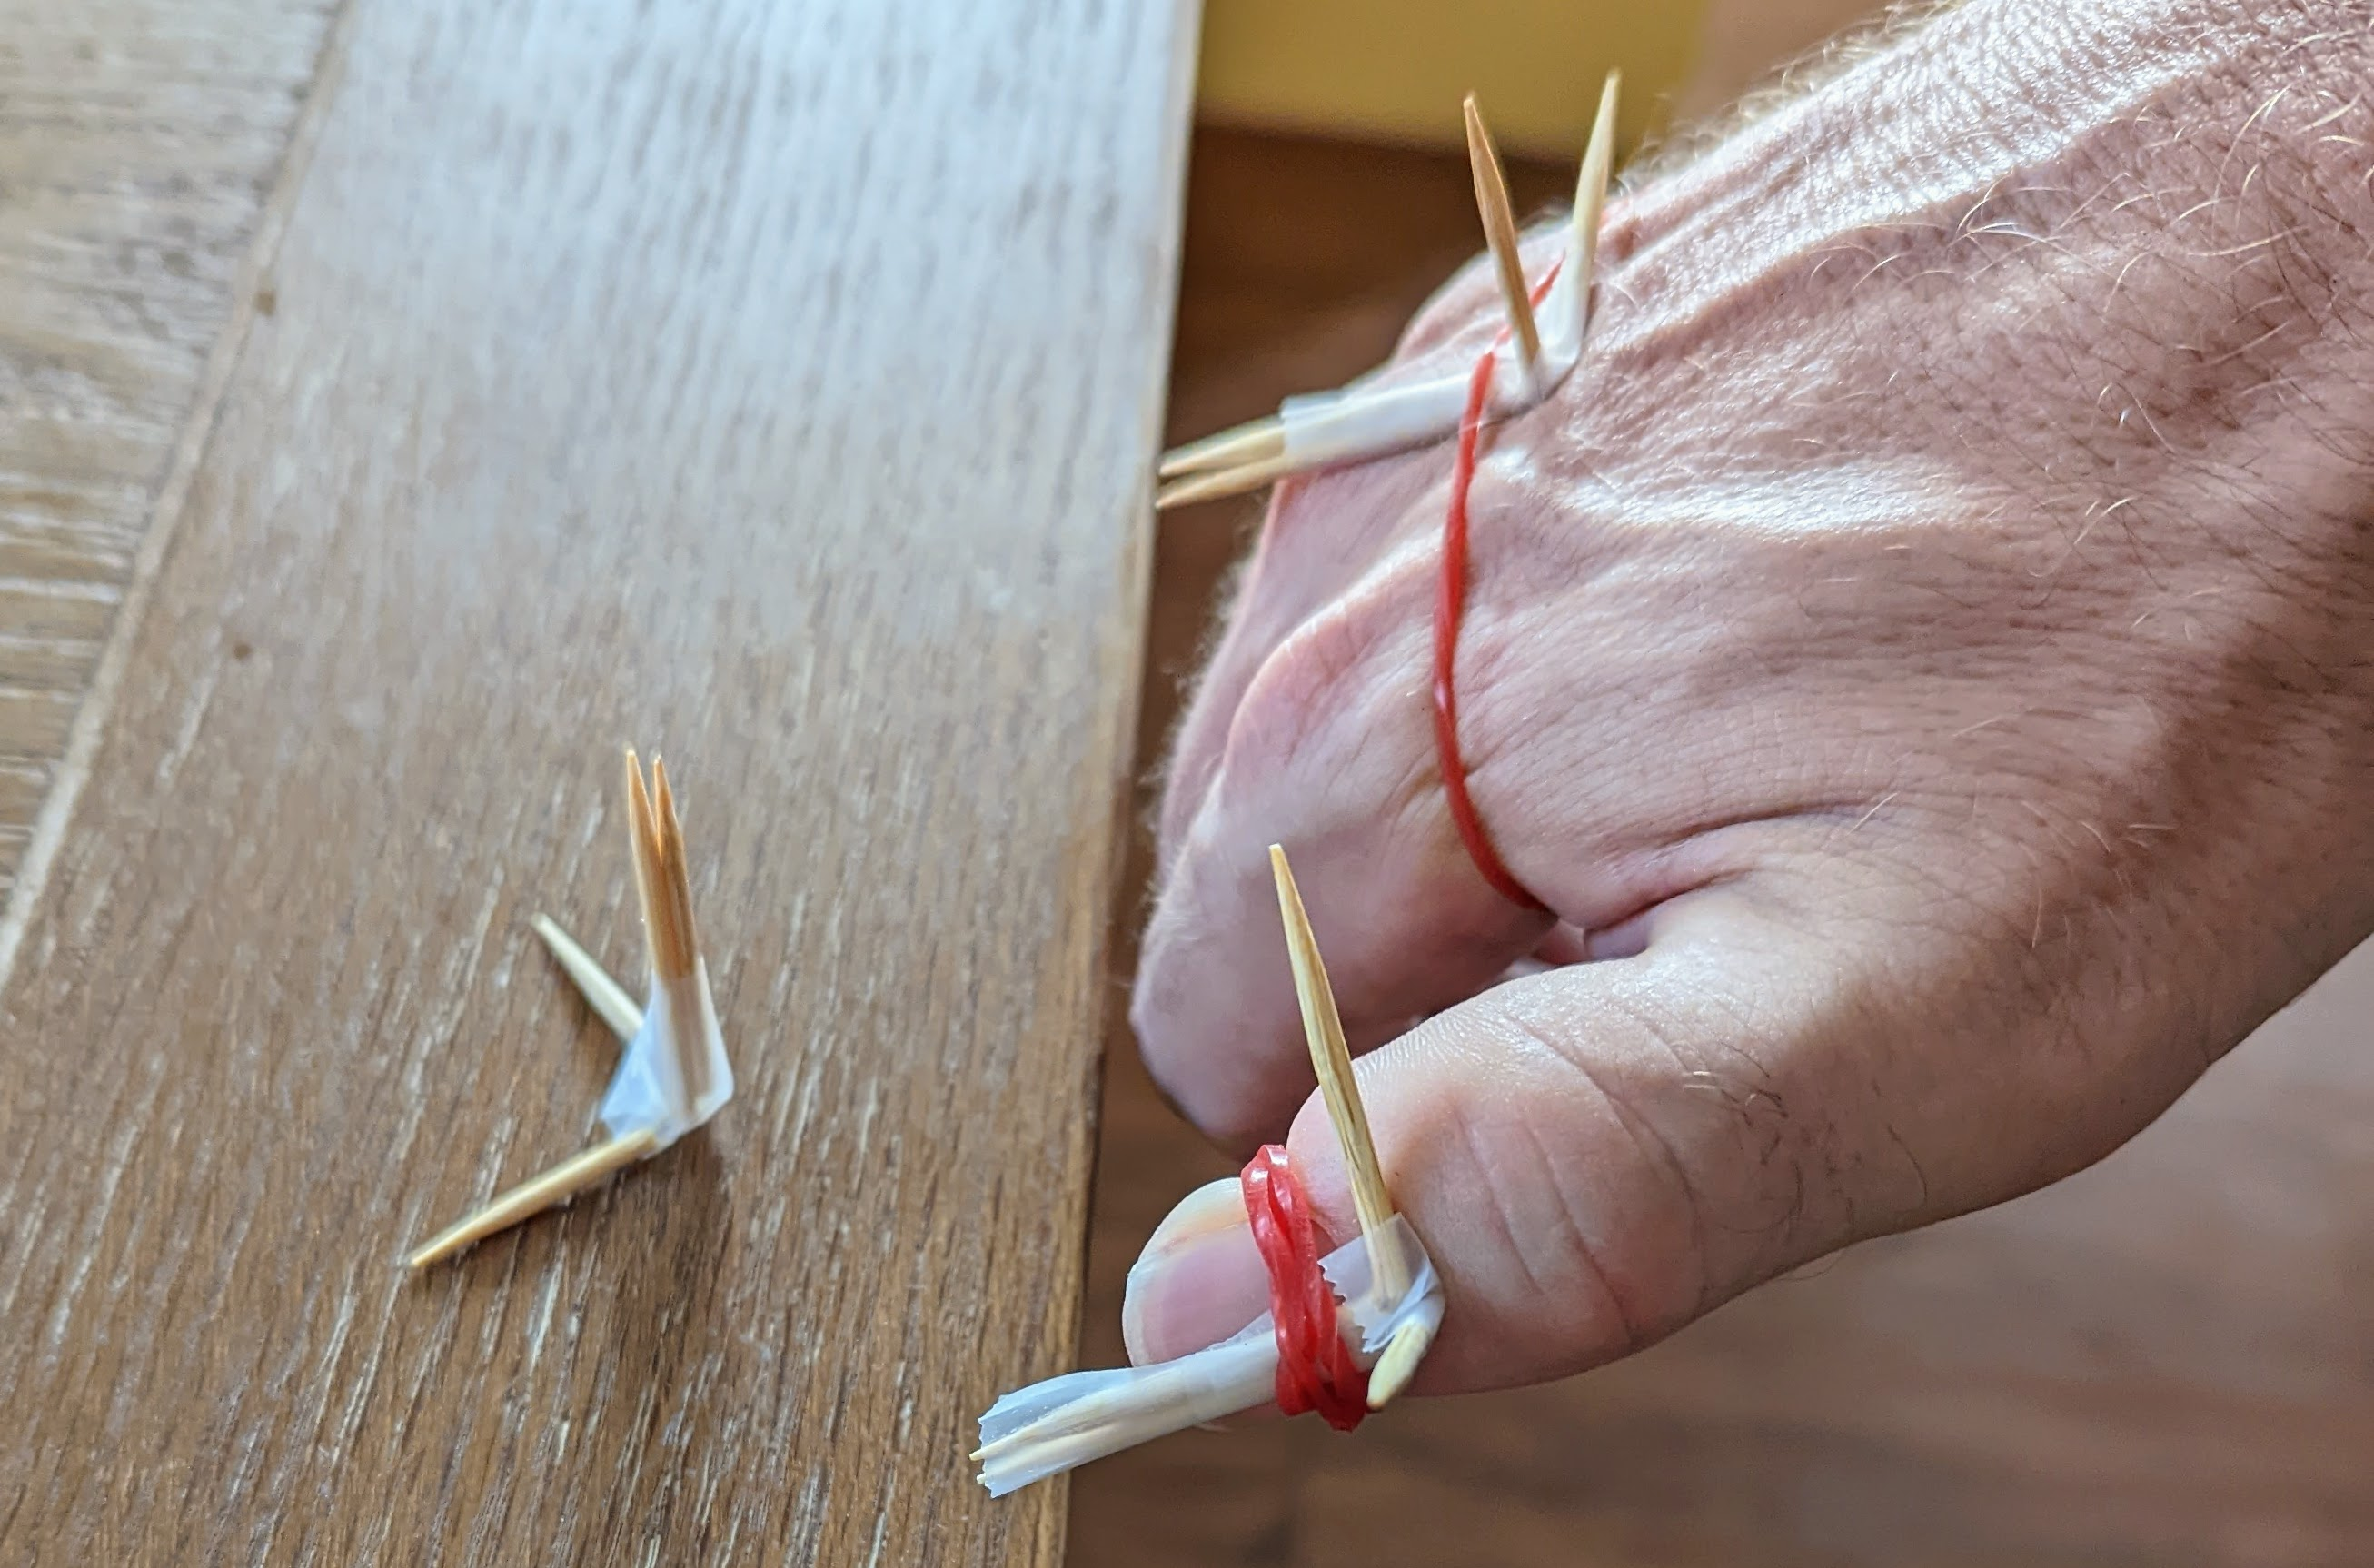
\includegraphics[width=10.41667in,height=\textheight]{images/hand.jpg}

}

\caption{\label{fig-hand}Rotations transform between coordinate system,
such as a fixed coordinate system in space (toothpicks on table), a body
centered coordinate system on the thumb and one on the plam.}

\end{figure}

\hypertarget{a-first-rotation}{%
\subsection{A first rotation}\label{a-first-rotation}}

Before we go into some math, lets have a first look how a rotation might
look like. On the left side you see data points in the original space.
On the right side a rotation by 45 degrees around the z-axis that have
been applied to the points. This rotation can be obtained by a rotation
matrix R:

\begin{Shaded}
\begin{Highlighting}[]
\NormalTok{R }\OtherTok{=} \FunctionTok{matrix}\NormalTok{(}\FunctionTok{c}\NormalTok{(}\FloatTok{0.7071068}\NormalTok{,  }\FloatTok{0.7071068}\NormalTok{,  }\FloatTok{0.0000000}\NormalTok{, }\SpecialCharTok{{-}}\FloatTok{0.7071068}\NormalTok{,  }\FloatTok{0.7071068}\NormalTok{,  }\FloatTok{0.0000000}\NormalTok{,  }\FloatTok{0.0000000}\NormalTok{,  }\FloatTok{0.0000000}\NormalTok{,  }\FloatTok{1.0000000}\NormalTok{), }\AttributeTok{nrow=}\DecValTok{3}\NormalTok{)}
\FunctionTok{round}\NormalTok{(R,}\DecValTok{4}\NormalTok{)}
\end{Highlighting}
\end{Shaded}

\begin{verbatim}
       [,1]    [,2] [,3]
[1,] 0.7071 -0.7071    0
[2,] 0.7071  0.7071    0
[3,] 0.0000  0.0000    1
\end{verbatim}

\begin{Shaded}
\begin{Highlighting}[]
\FunctionTok{par}\NormalTok{(}\AttributeTok{mfrow=}\FunctionTok{c}\NormalTok{(}\DecValTok{1}\NormalTok{,}\DecValTok{2}\NormalTok{))}
\end{Highlighting}
\end{Shaded}

As we will see in a second an example a point \(x\) of the rabid cloud
is transformed via:

\[
  x_\text{rot} = R \, x
\]

\begin{Shaded}
\begin{Highlighting}[]
\FunctionTok{p3d}\NormalTok{(rabbit, }\AttributeTok{h=}\ConstantTok{NULL}\NormalTok{, }\AttributeTok{xlab=}\StringTok{\textquotesingle{}x\textquotesingle{}}\NormalTok{, }\AttributeTok{ylab=}\StringTok{\textquotesingle{}y\textquotesingle{}}\NormalTok{, }\AttributeTok{zlab=}\StringTok{\textquotesingle{}z\textquotesingle{}}\NormalTok{, )}
\end{Highlighting}
\end{Shaded}

\begin{figure}[H]

{\centering 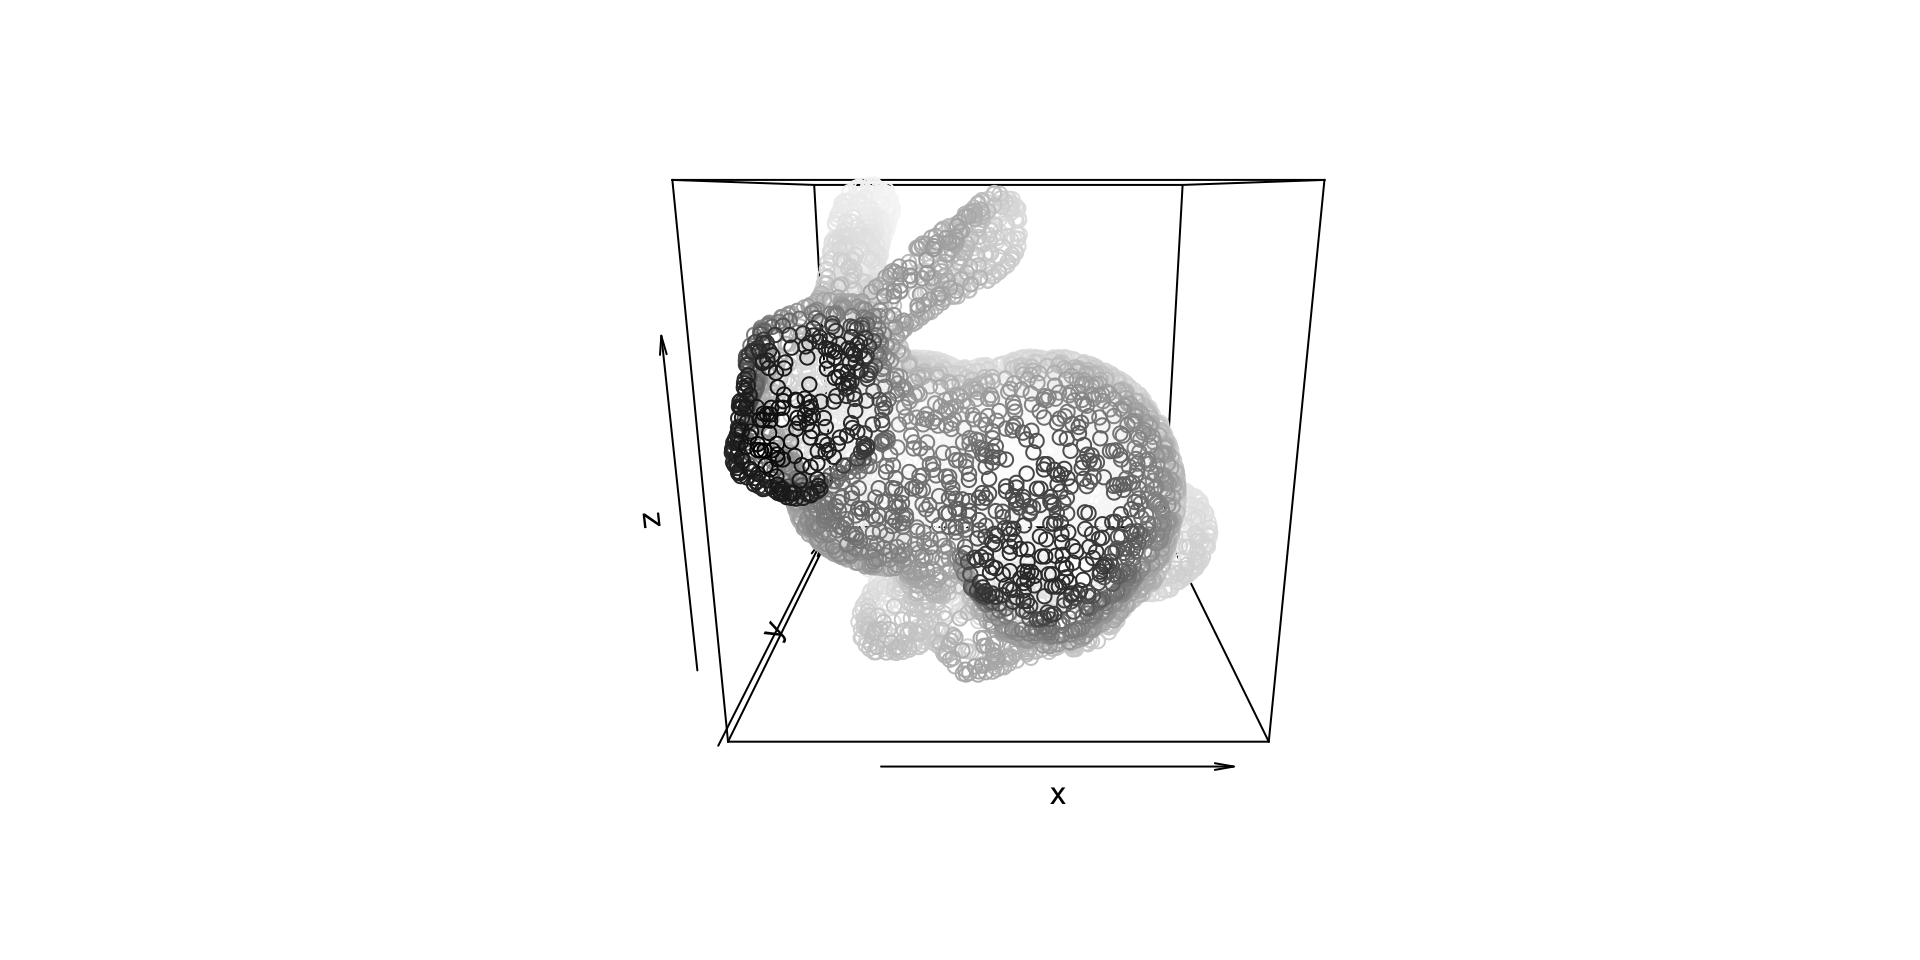
\includegraphics{Note_on_Quaternion_files/figure-pdf/rot-bunny-plot-1.pdf}

}

\caption{Left: orinial data. Right: data rotated by 45 degrees around
y-axis (or coordinate system rotated by -45) degrees. The y-axis points
up and the rotation is done in counter clock-wise manner}

\end{figure}

\begin{Shaded}
\begin{Highlighting}[]
\CommentTok{\#It\textquotesingle{}s vector times Matrix for row{-}vectors}
\CommentTok{\#Therefore we have to transpose (R x) to x\^{}T R\^{}T}
\FunctionTok{p3d}\NormalTok{(rabbit }\SpecialCharTok{\%*\%} \FunctionTok{t}\NormalTok{(R), }\AttributeTok{h=}\ConstantTok{NULL}\NormalTok{) }
\end{Highlighting}
\end{Shaded}

\begin{figure}[H]

{\centering 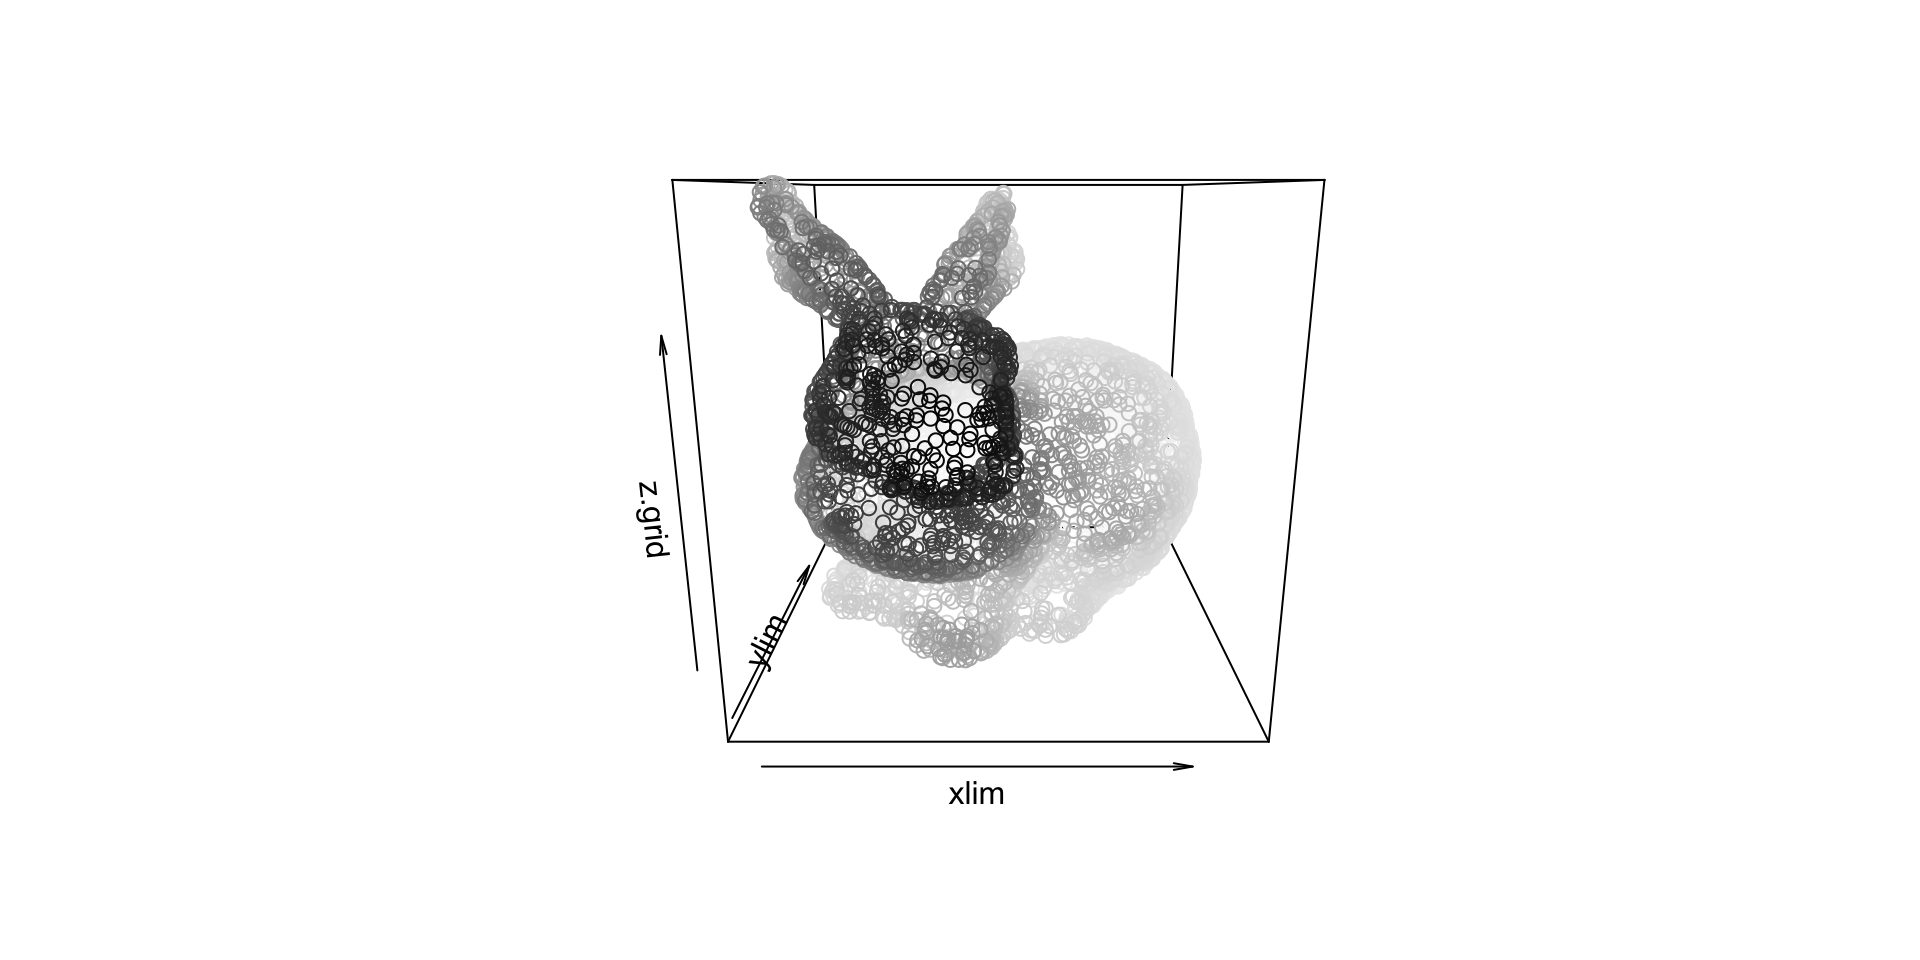
\includegraphics{Note_on_Quaternion_files/figure-pdf/rot-bunny-plot-2.pdf}

}

\caption{Left: orinial data. Right: data rotated by 45 degrees around
y-axis (or coordinate system rotated by -45) degrees. The y-axis points
up and the rotation is done in counter clock-wise manner}

\end{figure}

\begin{Shaded}
\begin{Highlighting}[]
\FunctionTok{par}\NormalTok{(}\AttributeTok{mfrow=}\FunctionTok{c}\NormalTok{(}\DecValTok{1}\NormalTok{,}\DecValTok{1}\NormalTok{))}
\end{Highlighting}
\end{Shaded}

\hypertarget{introduction}{%
\subsection{Introduction}\label{introduction}}

Rotations between rigid objects can be described as a linear
transformation from one coordinate system to another, with the same
origin. A first example is the bunny from above. Another similar example
of such a rotation is the orientation of your cell phone after you
picked it up compared to the position on the table, or the orientation
of the thumb in figure compared to the coordinate system of the palm.

A very illustrative example is an airplane which is at \(t=0\) on the
ground and is at \(t=t\) in the air. Besides the translation, the
orientation of the plane at \(t=0\) relative to the plane at \(t=t\) can
be described by a different heading (the \emph{yaw} angle) obtained
while taxing, the \emph{pitch} angle obtained in the climbing phase and
a rotation around the axis of flight the \emph{roll} angle. During this
phase many rotations happen but they can all be summarized in a single
rotation.

\hypertarget{parameterization}{%
\subsection{Parameterization}\label{parameterization}}

\hypertarget{definition-of-rotations}{%
\subsubsection{Definition of rotations}\label{definition-of-rotations}}

Rotations can be seen as linear transformation from one coordinate
system into another. But there are several way to parametrize them. The
first is via a rotation matrix.

\hypertarget{rotation-matrix-general-properties}{%
\subsubsection{Rotation matrix (general
properties)}\label{rotation-matrix-general-properties}}

In principal a rotation is given by the 9 matrix elements of \(R\).
However they cannot be arbitrary, they still need to describe rotations.
What are the defining properties of rotations? It turns out that a
rotation, has an inverse and the inverse simply the transposed
\(R^{-1} = R^T\) (this is the orthogonality). Further, \(det(R)=1\) this
is a consequence that the volume in the rotated system stays constant
and also the orientation (it's \(det(R)=1\) and not just
\(|det(d)|=1\)). So in matrix notation a rotation is defined by

\begin{equation}\protect\hypertarget{eq-rot}{}{
R=\begin{bmatrix}r_{11} & r_{12} & r_{13} \\r_{21} & r_{22} & r_{23} \\r_{31} & r_{32} & r_{33} \end{bmatrix}, \quad R^TR=RR^T=1,\quad det(R)=1  
}\label{eq-rot}\end{equation}

Multiplying two rotation matrices \(R_1\) and \(R_2\) is a again a
rotation matrix, this is why rotations in 3D are also called special
orthogonal group \texttt{SO(3)}. Note that the order of rotations matter
and \(R_1 R_2 \ne R_2 R_1\)

So it's obvious that is over parameterized using 9 values and there are
constrains on the \(r_{ij}\) so that eq. 1 is fulfilled.

\hypertarget{rotation-matrices-the-from-to-pitfall}{%
\paragraph{Rotation-Matrices (``the from to''
pitfall)}\label{rotation-matrices-the-from-to-pitfall}}

When we condescend ourselves to the depth of matrix multiplication, the
first of two pitfalls lingers around. This is due to the fact that
matrix multiplication introduces an order. Say, we want to transform a
vector \(\vec{f}\) from a ``from coordinate system'' into a vector
\(\vec{t}\) given in coordinates of the ``to coordinate system''. We can
do this via:

\[
\vec{t}=R \,\vec{f}
\]

To go the other way around, use \(\vec{f}=R^{-1} \vec{t}\). Figure XXX
gives an example.

\begin{figure}

{\centering 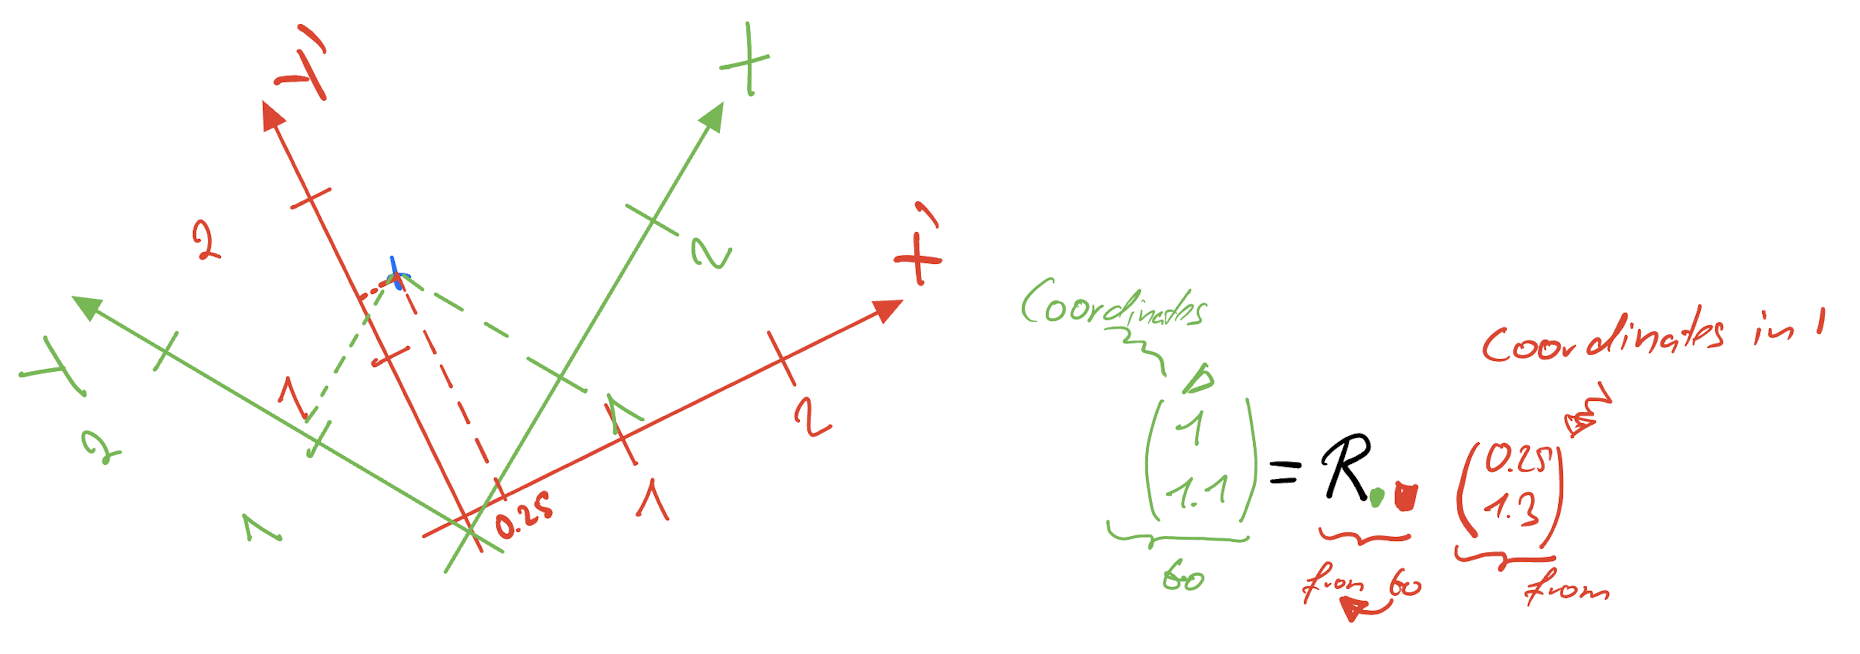
\includegraphics[width=10.41667in,height=\textheight]{images/from_to_in_2D.png}

}

\caption{\label{fig-fromto}A rotation, transforms the coordinates of a
point, from the red coordinate system into the green.}

\end{figure}

\hypertarget{the-body-and-the-lab-frame}{%
\paragraph{The body and the lab
frame}\label{the-body-and-the-lab-frame}}

Rotations are just transformation between to coordinate system. Some
coordinate system have special meanings. It's good to think of the
airplane again and think of two coordinate systems. One is fixed with
the airplane, this is called body frame one is fixed with the earth this
is called lab frame.

\begin{itemize}
\item
  In the \textbf{body frame} of points of the plane have the same x,y,z
  coordinates (if nothing bad happens), a plane is rigid body.
\item
  In the \textbf{lab frame} the gravity stays constant (it points down).
  People not sitting in the plane see the coordinates of the plane in
  this system.
\end{itemize}

\hypertarget{choosing-the-direction-of-the-rotation}{%
\paragraph{Choosing the direction of the
rotation}\label{choosing-the-direction-of-the-rotation}}

The question is with is the ``to system'' and which is the ``from
system''. As often when there is no mathematical reason for a certain
way to do things thinks get ugly. There is no natural way to choose one
over the other but for some applications a certain order is quite handy.

\begin{itemize}
\item
  \textbf{Body to Lab}: If you do visualizations, it is a least
  concepually nicer to describe the rotation from body to lab. Knowing
  the points of the airplane and the rotation, you can draw a picture of
  the rotated airplane.
\item
  \textbf{Lab to body} In the lab frame the gravity stays constant,
  often choosen in z-direction as \((0,0,-g)\), then knowing the
  rotation allows to calculate the gravity on the x-component of an IMU
  sensor in the plane.
\end{itemize}

This is an unnecessary source of confusion and some author even coin
different terms like \emph{rotations} and \emph{transformations} and
think of one coordinate system as the \emph{world coordinate system} or
lab system (Großekatthöfer and Yoon 2012). It is important to state the
direction of the transformation and ideally stick to that order. I find
it easier use \textbf{body to lab} and use this transformation.

\begin{tcolorbox}[enhanced jigsaw, opacitybacktitle=0.6, rightrule=.15mm, breakable, bottomtitle=1mm, arc=.35mm, colframe=quarto-callout-important-color-frame, coltitle=black, leftrule=.75mm, title=\textcolor{quarto-callout-important-color}{\faExclamation}\hspace{0.5em}{We use body to lab rotations in this text.}, left=2mm, toptitle=1mm, colbacktitle=quarto-callout-important-color!10!white, titlerule=0mm, colback=white, bottomrule=.15mm, toprule=.15mm, opacityback=0]

\end{tcolorbox}

\hypertarget{parameterization-using-elementary-rotation.}{%
\subsubsection{Parameterization using elementary
rotation.}\label{parameterization-using-elementary-rotation.}}

Many repeated rotations are again a rotation (closure). Moreover it can
be shown that an arbitrary rotation can be build out of three elementary
rotations. Here the mess begins, there are many ways to define such as
decomposition. For example one possibility is: First, a
counter-clockwise rotation \(R_z(\alpha)\) around the \(z\)-axis by an
angle of \(\alpha\). Second, \(R_x(\beta)\) rotates around ``the new''
\(x\)-axis and finally by \(R_z(\gamma)\) around the new \(z\)-axis.

\begin{figure}

{\centering 

\href{https://en.wikipedia.org/wiki/Euler_angles}{\includegraphics{images/Euler2a.gif}}

}

\caption{\label{fig-rot-ball}Animation showing the sequence of
elementary rotation. Taken from wikepedia}

\end{figure}

The animation in Figure~\ref{fig-rot-ball} shows three consecutive
rotations. Is is important not to forget that, we use column vector and
do matrix times vector hence. The complete rotation for first \(R_1\)
then \(R_2\) then \(R_3\) is written as

\begin{tcolorbox}[enhanced jigsaw, opacitybacktitle=0.6, rightrule=.15mm, breakable, bottomtitle=1mm, arc=.35mm, colframe=quarto-callout-caution-color-frame, coltitle=black, leftrule=.75mm, title=\textcolor{quarto-callout-caution-color}{\faFire}\hspace{0.5em}{Danger}, left=2mm, toptitle=1mm, colbacktitle=quarto-callout-caution-color!10!white, titlerule=0mm, colback=white, bottomrule=.15mm, toprule=.15mm, opacityback=0]
\[
R = R_3 R_2 R_1
\]
\end{tcolorbox}

Going the other way around is also possible, you just need to redefine
matrix multiplications.

\begin{tcolorbox}[enhanced jigsaw, opacitybacktitle=0.6, rightrule=.15mm, breakable, bottomtitle=1mm, arc=.35mm, colframe=quarto-callout-caution-color-frame, coltitle=black, leftrule=.75mm, title=\textcolor{quarto-callout-caution-color}{\faFire}\hspace{0.5em}{More details on the order.}, left=2mm, toptitle=1mm, colbacktitle=quarto-callout-caution-color!10!white, titlerule=0mm, colback=white, bottomrule=.15mm, toprule=.15mm, opacityback=0]
Here is an explanation (taken from stackexchange)

The product \(AB\) of matrices is the effect of applying \(A\) after
applying \(B\), simply because we write the ``effect'' of a matrix \(A\)
on a vector \(v\) as \(Av\) (i.e., the convention is to work with column
vectors). Thus \((AB)v = A(Bv)\) is \(A\) applied to \(Bv\). Note that
this convention matches the usual notation for (nested) functions:
\(\log(\sin(x))\) is the logarithm function applied to the result from
applying the sine function to \(x\).

Of course, the rules for computing the product of matrices are just
right for this convention. Or, if one wanted \(AB\) to stand for ``first
apply \(A\), then apply \(B\)'', one would use row vectors instead and
write ``A applied to \(v\)'' as \(vA\) - which is very uncommon (and in
effect just means that one works with the transposed matrices, relative
to the usual convention).
\end{tcolorbox}

\hypertarget{deriving-the-elementary-transformations}{%
\paragraph{Deriving the elementary
transformations}\label{deriving-the-elementary-transformations}}

The individual transformations can be derived by looking where the unit
vectors are transformed. In the figure below you see a derivation of the
rotation matrix \(R_z(\alpha)\) around the z axis with an angle of
\(\alpha>0\) . We move the body centric coordinate system w.r.t the
fixed system the direction is determined by the right-hand rule (thumb
show in direction of the rotation and fingers indicate the direction)

\begin{figure}

{\centering 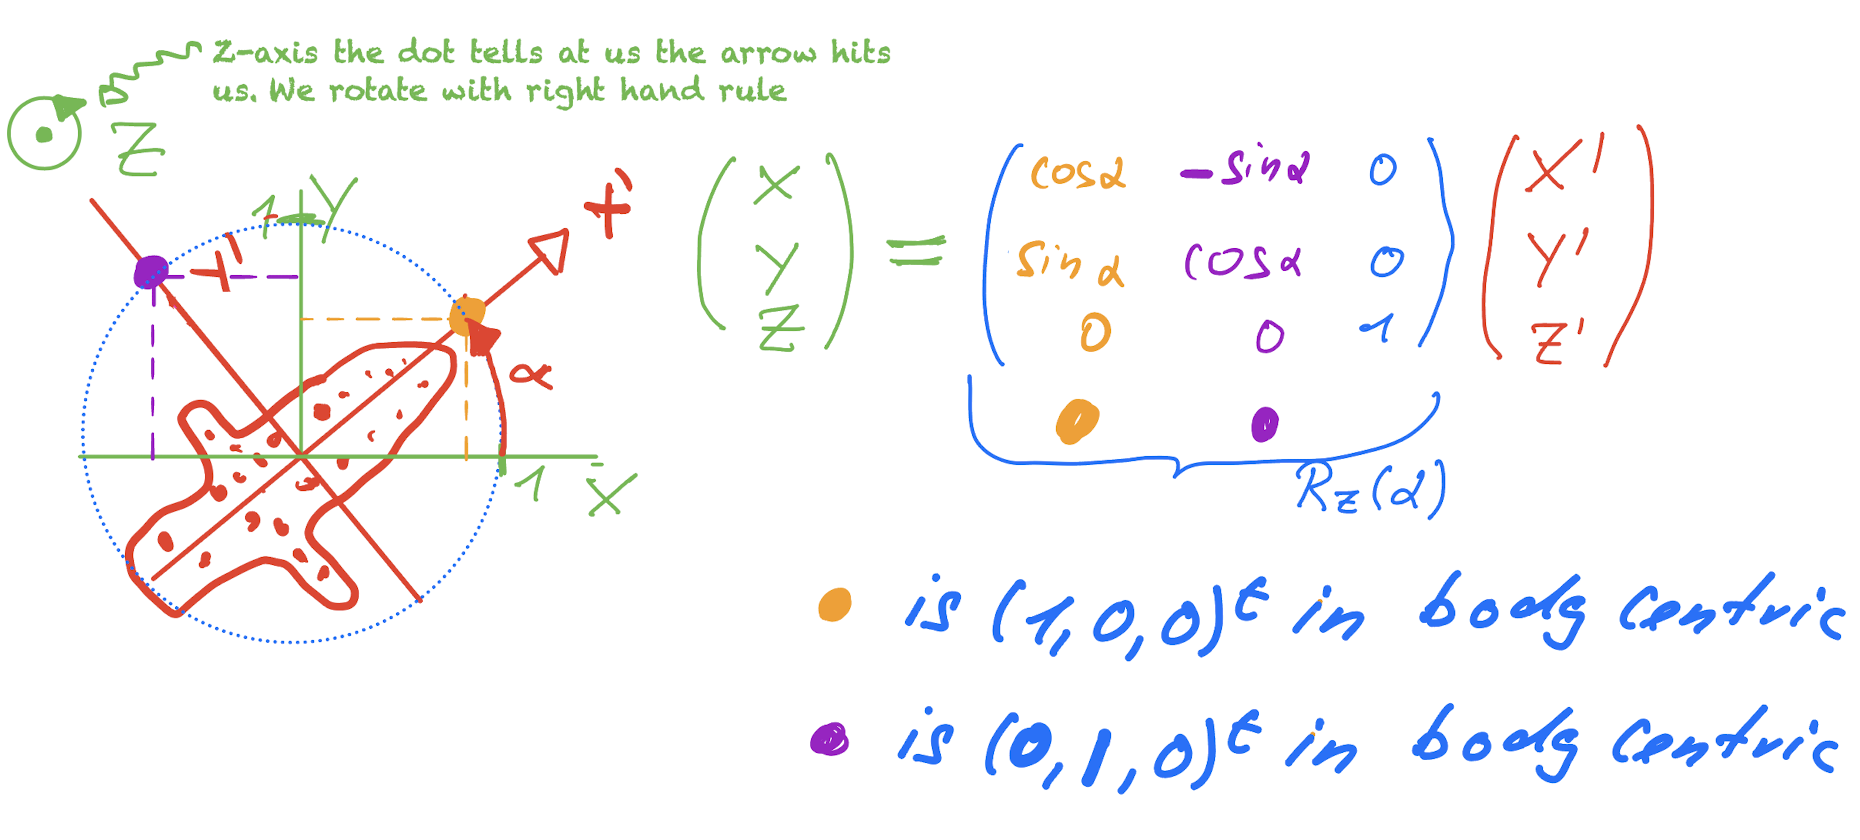
\includegraphics{images/rz_alpha.png}

}

\caption{Rotation around z-axis with positve \(\alpha\) the dots from
the airplane in the fixed body system.}

\end{figure}

So in this case we have for a rotation about \(\alpha\) around the
z-Axis.

\begin{equation}\protect\hypertarget{eq-yaw}{}{
  R_z(\alpha) = R_{L \leftarrow B}^z(\alpha) =\begin{bmatrix}\cos(\alpha) & -\sin(\alpha) & 0 \\\sin(\alpha) &\cos(\alpha) & 0 \\0 & 0 & 1 \end{bmatrix}
}\label{eq-yaw}\end{equation}

For moving the rabit , we get the following rotation matrix:

\begin{Shaded}
\begin{Highlighting}[]
\NormalTok{Rz }\OtherTok{=} \ControlFlowTok{function}\NormalTok{(a)\{}
  \FunctionTok{return}\NormalTok{(}
    \FunctionTok{matrix}\NormalTok{(}
        \FunctionTok{c}\NormalTok{(}\FunctionTok{cos}\NormalTok{(a), }\SpecialCharTok{{-}}\FunctionTok{sin}\NormalTok{(a), }\DecValTok{0}\NormalTok{, }\FunctionTok{sin}\NormalTok{(a), }\FunctionTok{cos}\NormalTok{(a), }\DecValTok{0}\NormalTok{, }\DecValTok{0}\NormalTok{, }\DecValTok{0}\NormalTok{, }\DecValTok{1}\NormalTok{)}
\NormalTok{        , }\AttributeTok{nrow=}\DecValTok{3}\NormalTok{, }\AttributeTok{byrow =}\NormalTok{ R}\SpecialCharTok{+}\ConstantTok{TRUE}\NormalTok{) }
\NormalTok{  )}
\NormalTok{\}}
\FunctionTok{Rz}\NormalTok{(}\DecValTok{45}\SpecialCharTok{*}\DecValTok{2}\SpecialCharTok{*}\NormalTok{pi}\SpecialCharTok{/}\DecValTok{360}\NormalTok{)}
\end{Highlighting}
\end{Shaded}

\begin{verbatim}
          [,1]       [,2] [,3]
[1,] 0.7071068 -0.7071068    0
[2,] 0.7071068  0.7071068    0
[3,] 0.0000000  0.0000000    1
\end{verbatim}

which is same rotation as used in the code used to transform the data.

\hypertarget{a-worked-out-example-yaw-pitch-roll}{%
\paragraph{A worked out example
(Yaw-Pitch-Roll)}\label{a-worked-out-example-yaw-pitch-roll}}

Using an airplane, we know what happens (taxiing, take-off, rolling) and
we can derive a nice chain of elementary rotations, which will serve as
reference for later. The derivation can also be found at the following
\href{https://www.dropbox.com/s/n3oc5fjwrn1zaiu/Rotations\%20without\%20tears.pdf?dl=0}{notes}.

In the example, we use the following angles

\begin{Shaded}
\begin{Highlighting}[]
\NormalTok{yaw }\OtherTok{=} \DecValTok{60} \SpecialCharTok{*} \DecValTok{2} \SpecialCharTok{*}\NormalTok{ pi }\SpecialCharTok{/} \DecValTok{360}     \CommentTok{\#This is w.r.t. the tower / labframe}
\NormalTok{pitch }\OtherTok{=} \SpecialCharTok{{-}}\DecValTok{50} \SpecialCharTok{*} \DecValTok{2} \SpecialCharTok{*}\NormalTok{ pi }\SpecialCharTok{/} \DecValTok{360}  \CommentTok{\#Angle of climb}
\NormalTok{roll }\OtherTok{=} \DecValTok{40} \SpecialCharTok{*} \DecValTok{2} \SpecialCharTok{*}\NormalTok{ pi }\SpecialCharTok{/} \DecValTok{360}    \CommentTok{\#Angle of roll}
\FunctionTok{print}\NormalTok{(}\FunctionTok{paste}\NormalTok{(}\StringTok{\textquotesingle{}In rad yaw \textquotesingle{}}\NormalTok{, yaw, }\StringTok{\textquotesingle{} pitch \textquotesingle{}}\NormalTok{, pitch, }\StringTok{\textquotesingle{} roll \textquotesingle{}}\NormalTok{,roll))}
\end{Highlighting}
\end{Shaded}

\begin{verbatim}
[1] "In rad yaw  1.0471975511966  pitch  -0.872664625997165  roll  0.698131700797732"
\end{verbatim}

The pitch needs to be negative in order that a the rotation leads to a
ascent (see later).

\hypertarget{taxiing-yaw-alpha}{%
\subparagraph{\texorpdfstring{Taxiing yaw
\(\alpha\)}{Taxiing yaw \textbackslash alpha}}\label{taxiing-yaw-alpha}}

For the given yaw we have:

\begin{Shaded}
\begin{Highlighting}[]
\NormalTok{R.yaw }\OtherTok{=} \FunctionTok{Rz}\NormalTok{(yaw) }
\NormalTok{R.yaw}
\end{Highlighting}
\end{Shaded}

\begin{verbatim}
          [,1]       [,2] [,3]
[1,] 0.5000000 -0.8660254    0
[2,] 0.8660254  0.5000000    0
[3,] 0.0000000  0.0000000    1
\end{verbatim}

\hypertarget{construction-of-data-points-for-the-airplane.}{%
\subparagraph{Construction of data points for the
airplane.}\label{construction-of-data-points-for-the-airplane.}}

We create \(3 \times N\) data points so that it is easier for plotting.
When we want to use the normal data points in statistics, we could use
vector times matrix and do proper transposing.

\begin{Shaded}
\begin{Highlighting}[]
\FunctionTok{set.seed}\NormalTok{(}\DecValTok{42}\NormalTok{)}
\NormalTok{n }\OtherTok{=} \DecValTok{1100}
\NormalTok{x }\OtherTok{=} \FunctionTok{runif}\NormalTok{(n,}\SpecialCharTok{{-}}\DecValTok{1}\NormalTok{,}\DecValTok{1}\NormalTok{)}
\NormalTok{y }\OtherTok{=} \FunctionTok{runif}\NormalTok{(n, }\SpecialCharTok{{-}}\FloatTok{0.4}\NormalTok{,}\FloatTok{0.4}\NormalTok{)}
\NormalTok{z }\OtherTok{=} \FunctionTok{runif}\NormalTok{(n,}\SpecialCharTok{{-}}\FloatTok{0.1}\NormalTok{,}\FloatTok{0.1}\NormalTok{)}
\NormalTok{col }\OtherTok{=} \FunctionTok{rep}\NormalTok{(}\StringTok{\textquotesingle{}blue\textquotesingle{}}\NormalTok{,n)}
\NormalTok{col[x}\SpecialCharTok{\textgreater{}}\FloatTok{0.5}\NormalTok{] }\OtherTok{=} \StringTok{\textquotesingle{}red\textquotesingle{}}
\NormalTok{col[x}\SpecialCharTok{\textless{}=} \SpecialCharTok{{-}}\FloatTok{0.5}\NormalTok{] }\OtherTok{=} \StringTok{\textquotesingle{}green\textquotesingle{}}
\NormalTok{col[y}\SpecialCharTok{\textless{}=} \SpecialCharTok{{-}}\FloatTok{0.2}\NormalTok{] }\OtherTok{=} \StringTok{\textquotesingle{}gray30\textquotesingle{}}

\NormalTok{plane }\OtherTok{=} \FunctionTok{as.matrix}\NormalTok{(}\FunctionTok{data.frame}\NormalTok{(}\AttributeTok{x=}\NormalTok{x,}\AttributeTok{y=}\NormalTok{y,}\AttributeTok{z=}\NormalTok{z))}
\NormalTok{plane }\OtherTok{=} \FunctionTok{t}\NormalTok{(plane) }\CommentTok{\#3xN}
\FunctionTok{library}\NormalTok{(rgl)}
\FunctionTok{library}\NormalTok{(scatterplot3d) }\CommentTok{\# load}
 

\NormalTok{make\_plot }\OtherTok{=} \ControlFlowTok{function}\NormalTok{(p1, p2, }\AttributeTok{l1=}\FunctionTok{c}\NormalTok{(}\StringTok{\textquotesingle{}x\textquotesingle{}}\NormalTok{,}\StringTok{\textquotesingle{}y\textquotesingle{}}\NormalTok{,}\StringTok{\textquotesingle{}z\textquotesingle{}}\NormalTok{), }\AttributeTok{l2=}\FunctionTok{c}\NormalTok{(}\StringTok{\textquotesingle{}x\textquotesingle{}}\NormalTok{,}\StringTok{\textquotesingle{}y\textquotesingle{}}\NormalTok{,}\StringTok{\textquotesingle{}z\textquotesingle{}}\NormalTok{), }\AttributeTok{angle =} \DecValTok{55}\NormalTok{) \{}
  \FunctionTok{par}\NormalTok{(}\AttributeTok{mfrow=}\FunctionTok{c}\NormalTok{(}\DecValTok{1}\NormalTok{,}\DecValTok{2}\NormalTok{))}
\NormalTok{  p1 }\OtherTok{=} \FunctionTok{t}\NormalTok{(p1)}
\NormalTok{  p2 }\OtherTok{=} \FunctionTok{t}\NormalTok{(p2)}
  \CommentTok{\#First plot}
  \FunctionTok{scatterplot3d}\NormalTok{(p1[,}\DecValTok{1}\NormalTok{],p1[,}\DecValTok{2}\NormalTok{],p1[,}\DecValTok{3}\NormalTok{], }
                \AttributeTok{xlim=}\FunctionTok{c}\NormalTok{(}\SpecialCharTok{{-}}\DecValTok{1}\NormalTok{,}\DecValTok{1}\NormalTok{), }\AttributeTok{ylim=}\FunctionTok{c}\NormalTok{(}\SpecialCharTok{{-}}\DecValTok{1}\NormalTok{,}\DecValTok{1}\NormalTok{), }\AttributeTok{zlim=}\FunctionTok{c}\NormalTok{(}\SpecialCharTok{{-}}\DecValTok{1}\NormalTok{,}\DecValTok{1}\NormalTok{), }
                \AttributeTok{color =}\NormalTok{ col,}
                \AttributeTok{xlab=}\NormalTok{l1[}\DecValTok{1}\NormalTok{], }\AttributeTok{ylab=}\NormalTok{l1[}\DecValTok{2}\NormalTok{], }\AttributeTok{zlab =}\NormalTok{ l1[}\DecValTok{3}\NormalTok{],}\AttributeTok{angle =}\NormalTok{ angle, }\AttributeTok{pch=}\DecValTok{16}\NormalTok{)}
  \FunctionTok{scatterplot3d}\NormalTok{(p2[,}\DecValTok{1}\NormalTok{],p2[,}\DecValTok{2}\NormalTok{],p2[,}\DecValTok{3}\NormalTok{], }
                \AttributeTok{xlim=}\FunctionTok{c}\NormalTok{(}\SpecialCharTok{{-}}\DecValTok{1}\NormalTok{,}\DecValTok{1}\NormalTok{), }\AttributeTok{ylim=}\FunctionTok{c}\NormalTok{(}\SpecialCharTok{{-}}\DecValTok{1}\NormalTok{,}\DecValTok{1}\NormalTok{), }\AttributeTok{zlim=}\FunctionTok{c}\NormalTok{(}\SpecialCharTok{{-}}\DecValTok{1}\NormalTok{,}\DecValTok{1}\NormalTok{), }
                \AttributeTok{color =}\NormalTok{ col,}
                \AttributeTok{xlab=}\NormalTok{l2[}\DecValTok{1}\NormalTok{], }\AttributeTok{ylab=}\NormalTok{l2[}\DecValTok{2}\NormalTok{], }\AttributeTok{zlab =}\NormalTok{ l2[}\DecValTok{3}\NormalTok{],}\AttributeTok{angle =}\NormalTok{ angle, }\AttributeTok{pch=}\DecValTok{16}\NormalTok{)}
\NormalTok{\}}
\end{Highlighting}
\end{Shaded}

To visualize, we need the body coordinates, transformed to lab
coordinates.

\begin{Shaded}
\begin{Highlighting}[]
\DocumentationTok{\#\#Since we have column vector, we have to transpose once more yielding}
\NormalTok{plane.yaw  }\OtherTok{=}\NormalTok{ R.yaw }\SpecialCharTok{\%*\%}\NormalTok{ plane }
\FunctionTok{make\_plot}\NormalTok{(plane, plane.yaw, }\AttributeTok{l2=}\FunctionTok{c}\NormalTok{(}\StringTok{"x\textquotesingle{}"}\NormalTok{,}\StringTok{"y\textquotesingle{}"}\NormalTok{,}\StringTok{"z\textquotesingle{}"}\NormalTok{))}
\end{Highlighting}
\end{Shaded}

\begin{figure}[H]

{\centering 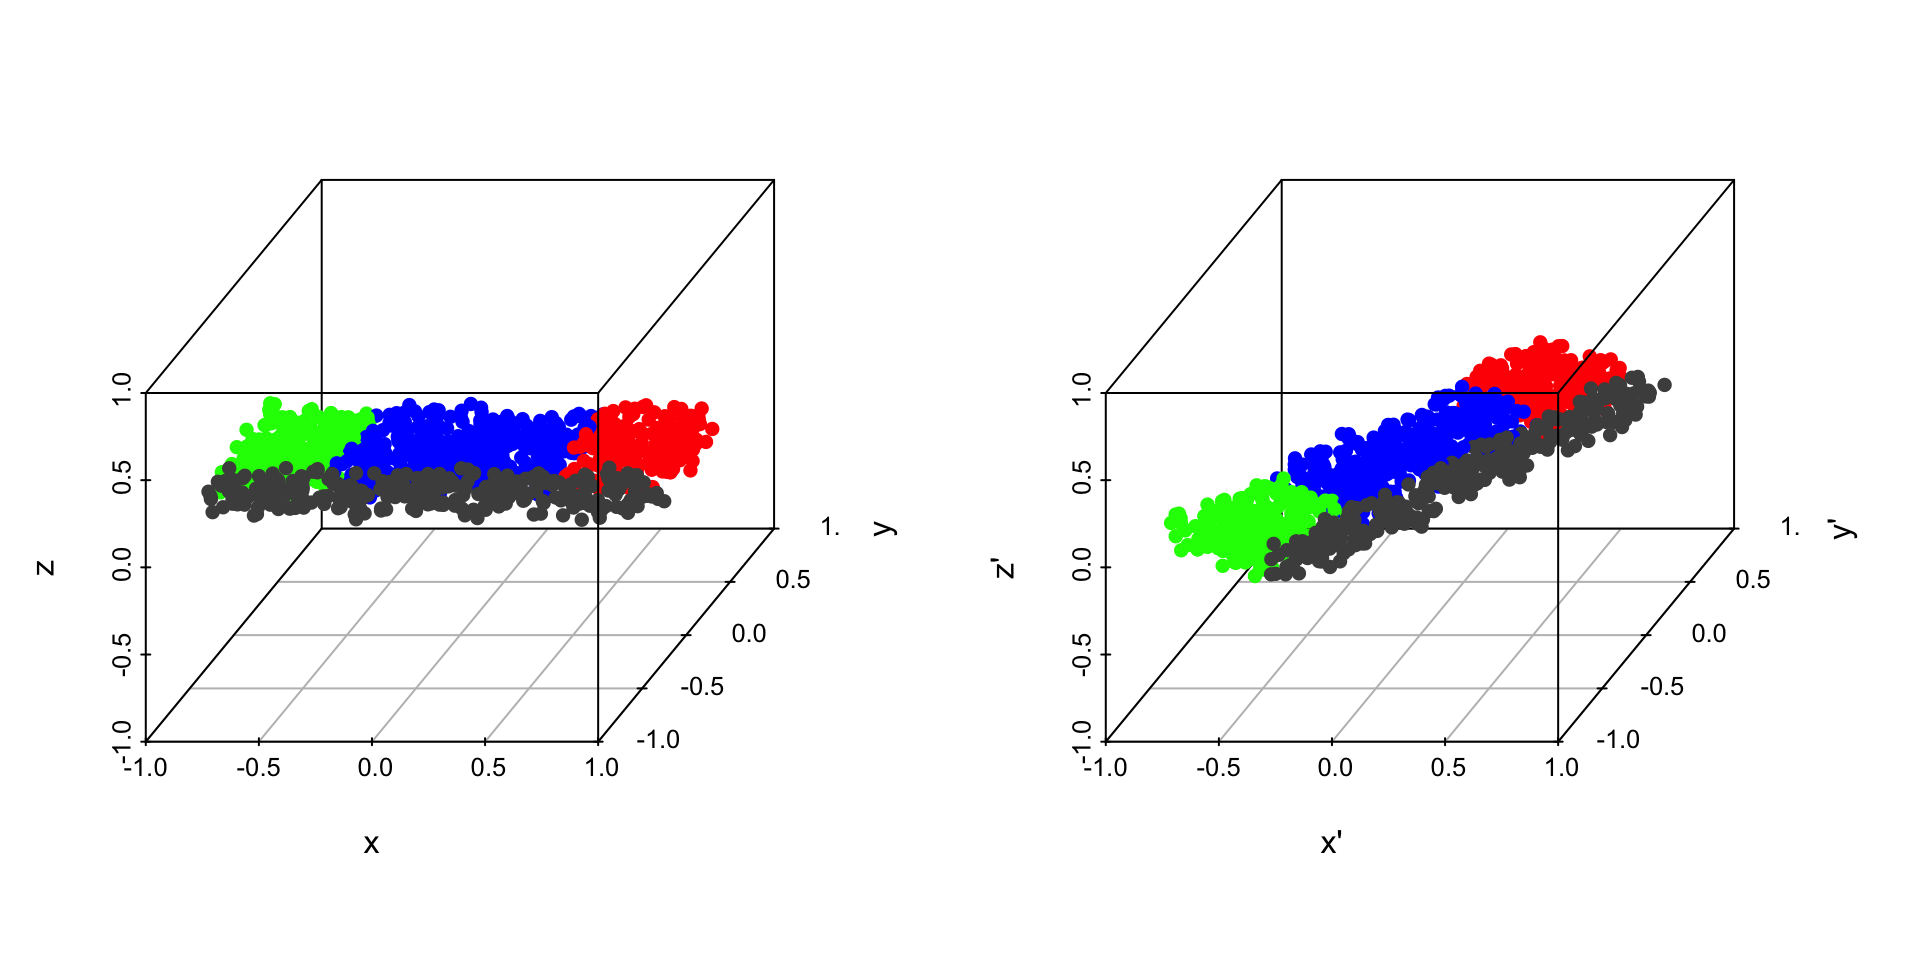
\includegraphics{Note_on_Quaternion_files/figure-pdf/yaw-plane-1.pdf}

}

\caption{Left: orinial data. Right: data rotated by yaw degrees around
z-axis}

\end{figure}

\begin{Shaded}
\begin{Highlighting}[]
\ControlFlowTok{if}\NormalTok{ (}\ConstantTok{FALSE}\NormalTok{)\{}\CommentTok{\#Debuggin}
  \FunctionTok{print}\NormalTok{(}\StringTok{\textquotesingle{}Maximal difference, in x{-}direction\textquotesingle{}}\NormalTok{)}
  \FunctionTok{max}\NormalTok{(}\FunctionTok{abs}\NormalTok{(plane.yaw[,}\DecValTok{3}\NormalTok{] }\SpecialCharTok{{-}}\NormalTok{ plane[,}\DecValTok{3}\NormalTok{]))}
\NormalTok{\}}
\end{Highlighting}
\end{Shaded}

\hypertarget{take-off-the-pitch-beta}{%
\subparagraph{\texorpdfstring{Take-off the pitch
\(\beta\)}{Take-off the pitch \textbackslash beta}}\label{take-off-the-pitch-beta}}

When the plane takes off, all rotates rotated about \(\beta\) about the
y-axis. This is given by

\[
  R^y(\beta) = \begin{bmatrix}\cos(\beta) & 0 & +\sin(\beta)\\
   0 & 1 & 0 \\
  -\sin(\beta) & 0 & \cos(\beta)\end{bmatrix}
\]

Note that the rotation is about the y-axis (use the right hand the thumb
is the axis and the fingers shows the direction). Acceding, corresponds
to negative values (that's the reason we choose negative value)

\begin{Shaded}
\begin{Highlighting}[]
\NormalTok{Ry }\OtherTok{=} \ControlFlowTok{function}\NormalTok{(b) }\FunctionTok{matrix}\NormalTok{(}
      \FunctionTok{c}\NormalTok{(}\FunctionTok{cos}\NormalTok{(b), }\DecValTok{0}\NormalTok{, }\SpecialCharTok{+}\FunctionTok{sin}\NormalTok{(b), }\DecValTok{0}\NormalTok{, }\DecValTok{1}\NormalTok{, }\DecValTok{0}\NormalTok{, }\SpecialCharTok{{-}}\FunctionTok{sin}\NormalTok{(b), }\DecValTok{0}\NormalTok{, }\FunctionTok{cos}\NormalTok{(b))}
\NormalTok{      , }\AttributeTok{nrow=}\DecValTok{3}\NormalTok{, }\AttributeTok{byrow =} \ConstantTok{TRUE}\NormalTok{) }
\NormalTok{R.pitch }\OtherTok{=} \FunctionTok{Ry}\NormalTok{(pitch) }
\NormalTok{R.pitch}
\end{Highlighting}
\end{Shaded}

\begin{verbatim}
          [,1] [,2]       [,3]
[1,] 0.6427876    0 -0.7660444
[2,] 0.0000000    1  0.0000000
[3,] 0.7660444    0  0.6427876
\end{verbatim}

Takeoff without taxiing

\begin{Shaded}
\begin{Highlighting}[]
\FunctionTok{make\_plot}\NormalTok{(plane, R.pitch }\SpecialCharTok{\%*\%}\NormalTok{ plane)}
\end{Highlighting}
\end{Shaded}

\begin{figure}[H]

{\centering 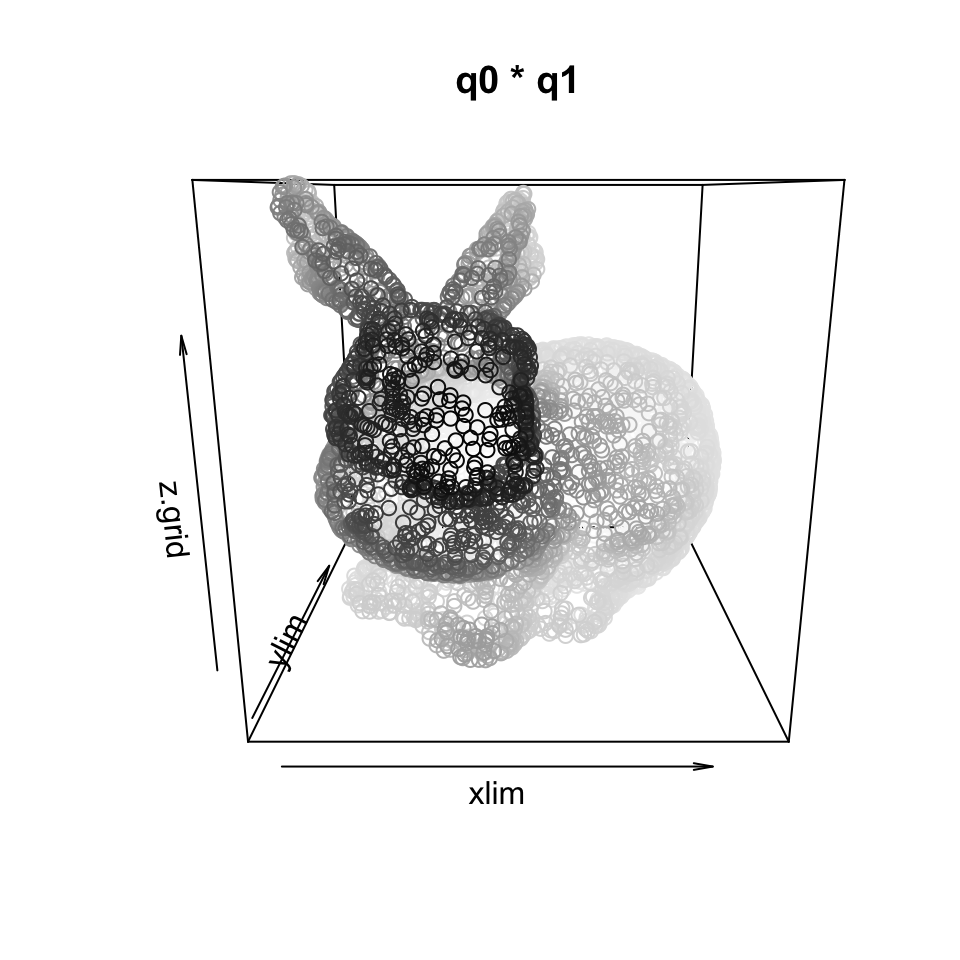
\includegraphics{Note_on_Quaternion_files/figure-pdf/unnamed-chunk-8-1.pdf}

}

\caption{Left: orinial data. Right: data rotated by XXX degrees around
y-axis}

\end{figure}

Takeoff with taxiing

Here, we combine the transformations (\textbf{note the order})

\[
x=R^{y}(\beta)R^z(\alpha)x'
\]

\begin{Shaded}
\begin{Highlighting}[]
\NormalTok{R }\OtherTok{=}\NormalTok{ R.pitch }\SpecialCharTok{\%*\%}\NormalTok{ R.yaw}
\NormalTok{plane.pitch.yaw }\OtherTok{=}\NormalTok{ R }\SpecialCharTok{\%*\%}\NormalTok{ plane }
\FunctionTok{make\_plot}\NormalTok{(plane.yaw, plane.pitch.yaw,}\AttributeTok{l1=}\FunctionTok{c}\NormalTok{(}\StringTok{"x\textquotesingle{}"}\NormalTok{, }\StringTok{"y\textquotesingle{}"}\NormalTok{, }\StringTok{"z\textquotesingle{}\textquotesingle{}"}\NormalTok{), }\AttributeTok{l2=}\FunctionTok{c}\NormalTok{(}\StringTok{"x\textquotesingle{}\textquotesingle{}"}\NormalTok{, }\StringTok{"y\textquotesingle{}\textquotesingle{}"}\NormalTok{, }\StringTok{"z\textquotesingle{}\textquotesingle{}"}\NormalTok{)) }
\end{Highlighting}
\end{Shaded}

\begin{figure}[H]

{\centering 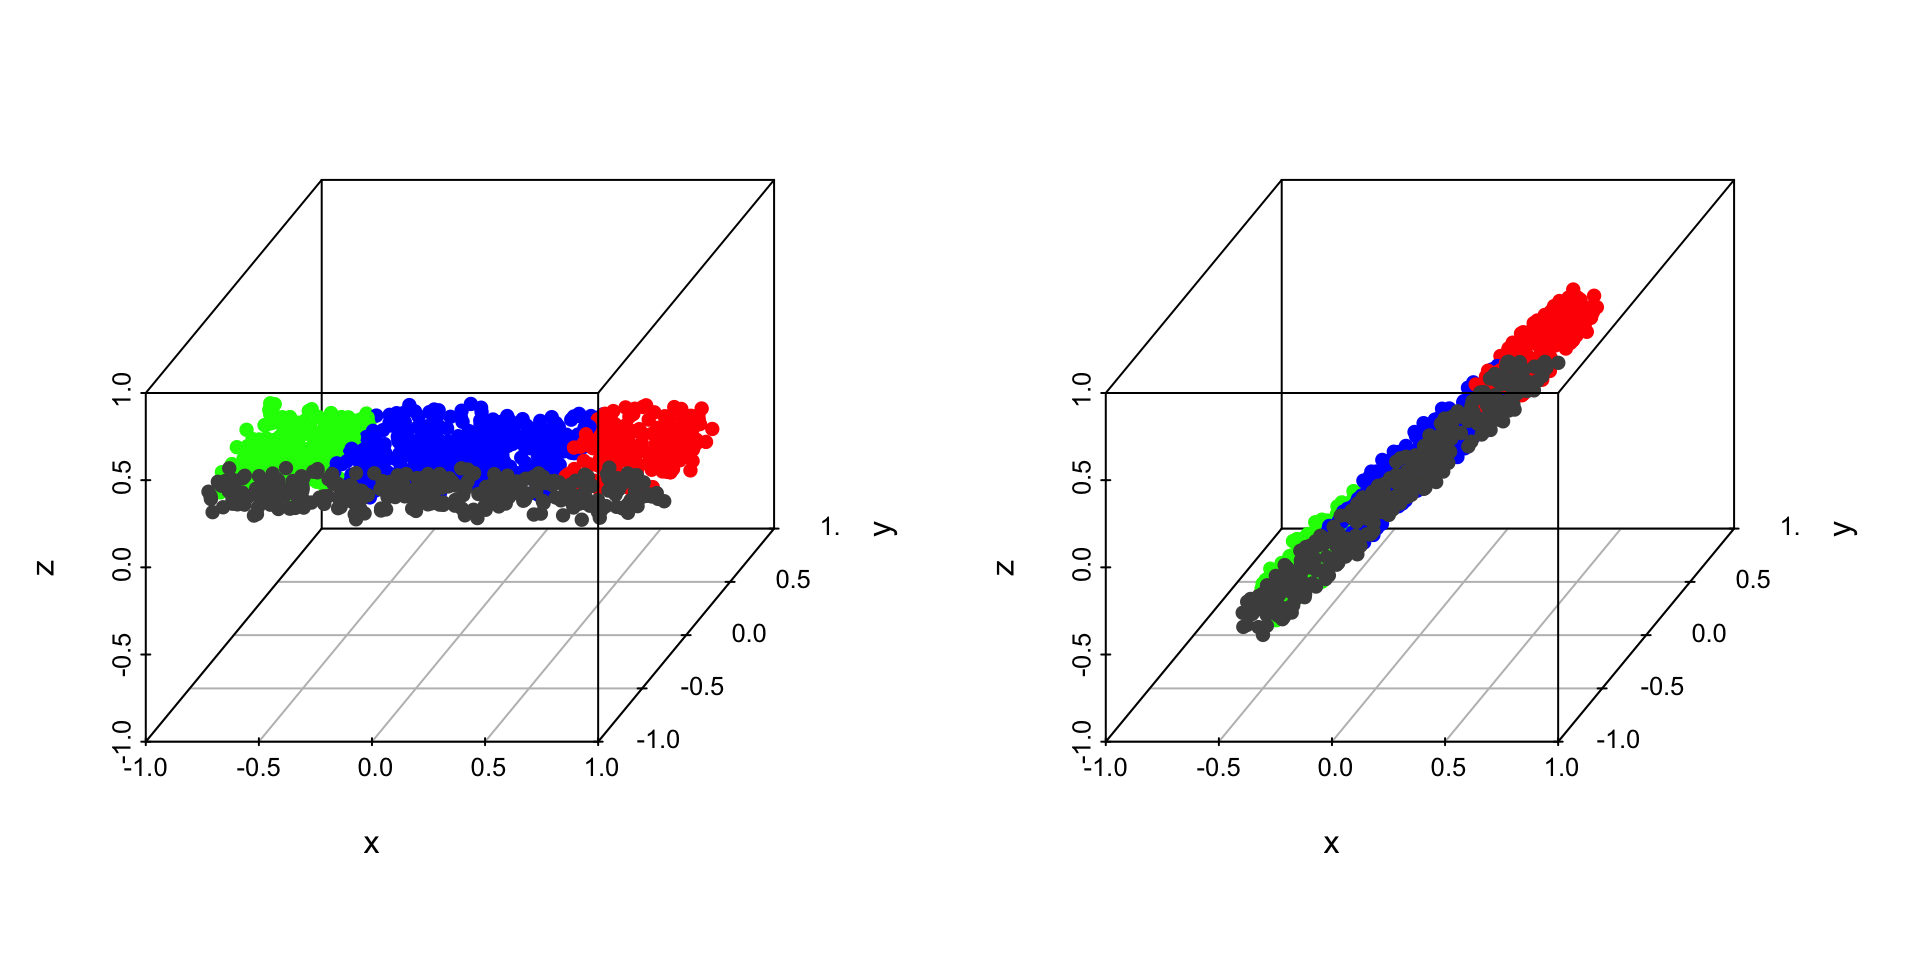
\includegraphics{Note_on_Quaternion_files/figure-pdf/unnamed-chunk-10-1.pdf}

}

\caption{Left: orinial data. Right: data rotated by XXX degrees around
y-axis}

\end{figure}

\begin{Shaded}
\begin{Highlighting}[]
\CommentTok{\#plot3d(plane.pitch.yaw[,1],plane.pitch.yaw[,2],plane.pitch.yaw[,3], xlim=c({-}1,1), ylim=c({-}1,1), zlim=c({-}1,1), col=col) }
\CommentTok{\#rglwidget()}
\end{Highlighting}
\end{Shaded}

\hypertarget{in-the-air-the-roll-gamma}{%
\subparagraph{\texorpdfstring{In the air, the roll
\(\gamma\)}{In the air, the roll \textbackslash gamma}}\label{in-the-air-the-roll-gamma}}

Now that we are in the air, we roll the plane about a certain degree
around the x-axis. This can be done by

\[
R^x(\gamma) = \begin{bmatrix}
1 & 0 & 0\\
0 & \cos(\gamma) & -\sin(\gamma) \\
 0 & \sin(\gamma) & \cos(\gamma) \end{bmatrix}
\]

\begin{Shaded}
\begin{Highlighting}[]
\NormalTok{Rx }\OtherTok{=} \ControlFlowTok{function}\NormalTok{(g) }\FunctionTok{matrix}\NormalTok{(}
      \FunctionTok{c}\NormalTok{(}\DecValTok{1}\NormalTok{,}\DecValTok{0}\NormalTok{,}\DecValTok{0}\NormalTok{, }\DecValTok{0}\NormalTok{, }\FunctionTok{cos}\NormalTok{(g), }\SpecialCharTok{{-}}\FunctionTok{sin}\NormalTok{(g), }\DecValTok{0}\NormalTok{, }\FunctionTok{sin}\NormalTok{(g), }\FunctionTok{cos}\NormalTok{(g))}
\NormalTok{      , }\AttributeTok{nrow=}\DecValTok{3}\NormalTok{, }\AttributeTok{byrow =} \ConstantTok{TRUE}\NormalTok{) }
\NormalTok{R.roll}\OtherTok{=}\FunctionTok{Rx}\NormalTok{(roll)}
\NormalTok{R.roll}
\end{Highlighting}
\end{Shaded}

\begin{verbatim}
     [,1]      [,2]       [,3]
[1,]    1 0.0000000  0.0000000
[2,]    0 0.7660444 -0.6427876
[3,]    0 0.6427876  0.7660444
\end{verbatim}

\hfill\break
The final transformation can be found via

\[
x=R(\alpha, \beta, \gamma)\,x= R^{x}(\gamma) R^{y}(\beta)\,R^z(\alpha)x'
\]

\begin{Shaded}
\begin{Highlighting}[]
\NormalTok{R }\OtherTok{=}\NormalTok{ R.roll }\SpecialCharTok{\%*\%}\NormalTok{ R.pitch }\SpecialCharTok{\%*\%}\NormalTok{ R.yaw}
\NormalTok{plane.roll.pitch.yaw }\OtherTok{=}\NormalTok{ R }\SpecialCharTok{\%*\%}\NormalTok{ plane }
\FunctionTok{make\_plot}\NormalTok{(plane.pitch.yaw, plane.roll.pitch.yaw,}\AttributeTok{l1=}\FunctionTok{c}\NormalTok{(}\StringTok{"x\textquotesingle{}\textquotesingle{}"}\NormalTok{, }\StringTok{"y\textquotesingle{}\textquotesingle{}"}\NormalTok{, }\StringTok{"z\textquotesingle{}\textquotesingle{}"}\NormalTok{), }\AttributeTok{l2=}\FunctionTok{c}\NormalTok{(}\StringTok{"x\textquotesingle{}\textquotesingle{}\textquotesingle{}"}\NormalTok{, }\StringTok{"y\textquotesingle{}\textquotesingle{}\textquotesingle{}"}\NormalTok{, }\StringTok{"z\textquotesingle{}\textquotesingle{}\textquotesingle{}"}\NormalTok{)) }
\end{Highlighting}
\end{Shaded}

\begin{figure}[H]

{\centering 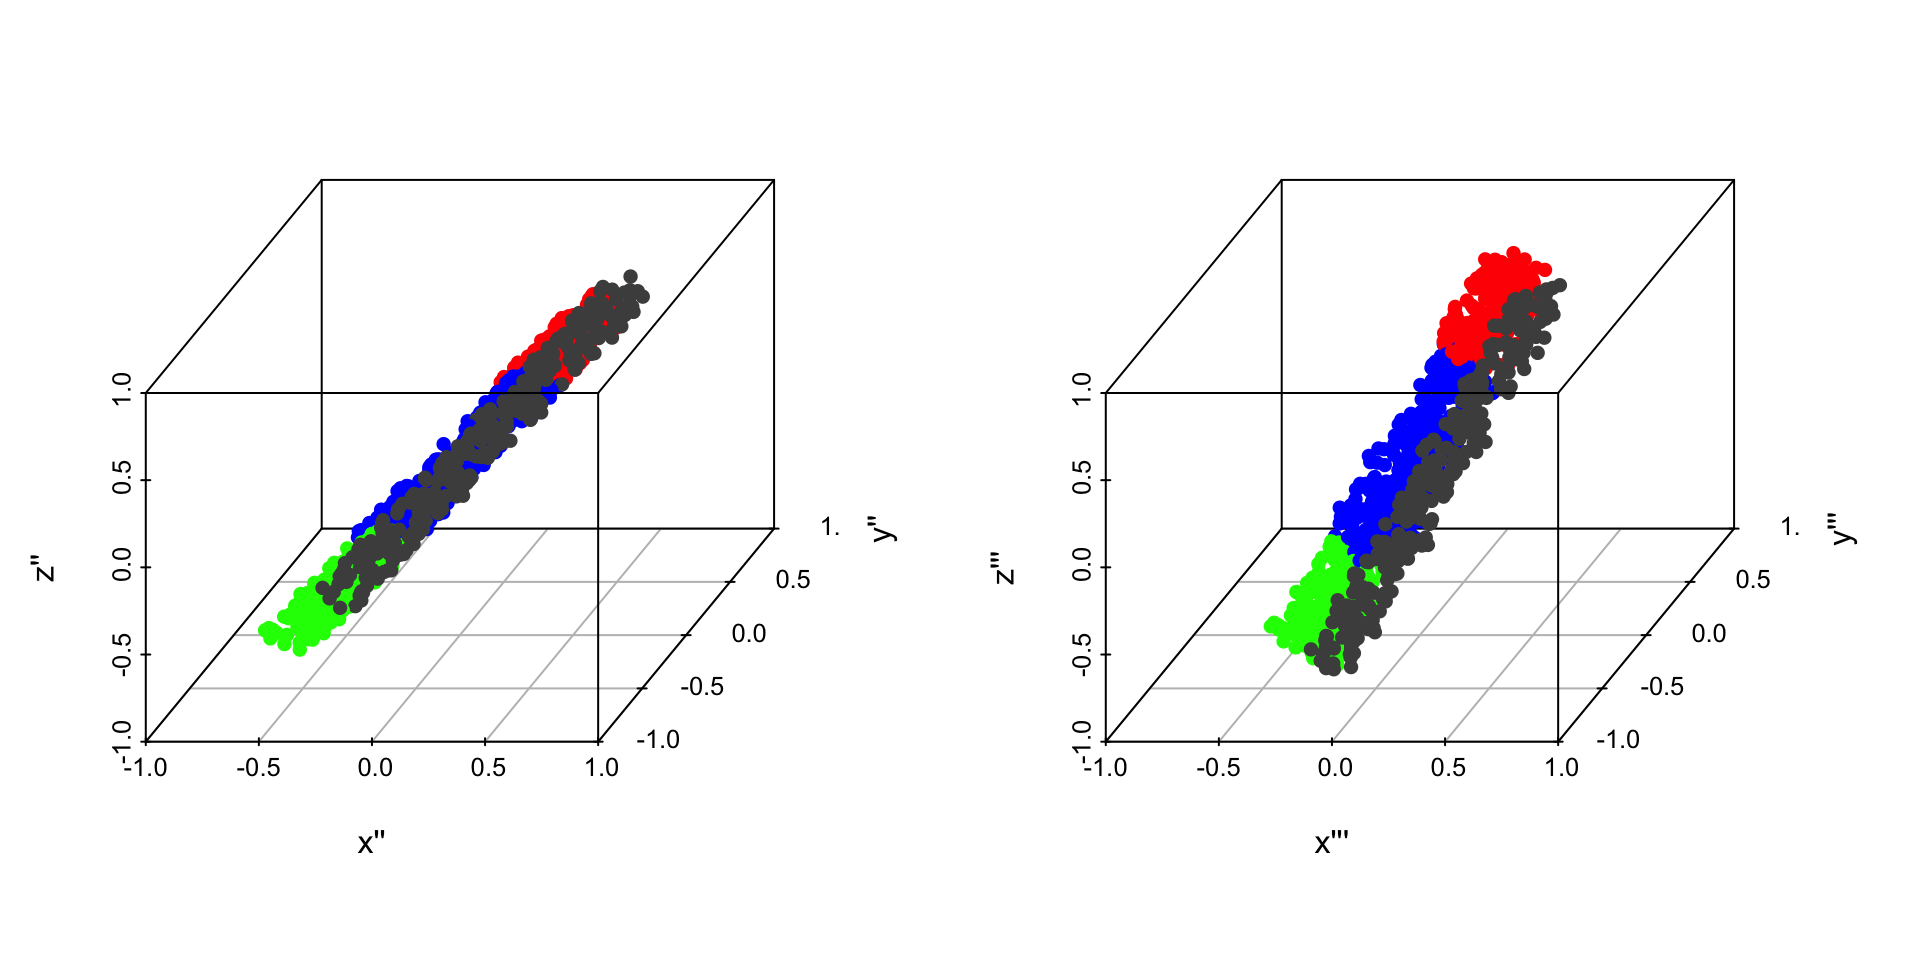
\includegraphics{Note_on_Quaternion_files/figure-pdf/comp_trafo-1.pdf}

}

\caption{Left: orinial data. Right: data rotated by degrees around
y-axis}

\end{figure}

Playing around (sorry not in document yet)

\begin{Shaded}
\begin{Highlighting}[]
\CommentTok{\#Return the rotion matrix (Lab  \textless{}{-} Fixed)}
\NormalTok{get\_R }\OtherTok{=} \ControlFlowTok{function}\NormalTok{(yaw, roll, pitch)\{}
\NormalTok{   Rroll }\OtherTok{=} \FunctionTok{Rx}\NormalTok{(roll)}
\NormalTok{   Ryaw  }\OtherTok{=} \FunctionTok{Rz}\NormalTok{(yaw)}
\NormalTok{   Rp }\OtherTok{=} \FunctionTok{Ry}\NormalTok{(pitch) }
\NormalTok{   Rani }\OtherTok{=}\NormalTok{ Rroll }\SpecialCharTok{\%*\%}\NormalTok{ Rp }\SpecialCharTok{\%*\%}\NormalTok{ Ryaw}
   \FunctionTok{return}\NormalTok{(Rani)}
\NormalTok{\}}
\FunctionTok{get\_R}\NormalTok{(yaw, roll, pitch)}
\end{Highlighting}
\end{Shaded}

\begin{verbatim}
          [,1]       [,2]       [,3]
[1,] 0.3213938 -0.5566704 -0.7660444
[2,] 0.4172120  0.8094565 -0.4131759
[3,] 0.8500824 -0.1868108  0.4924039
\end{verbatim}

\begin{Shaded}
\begin{Highlighting}[]
\ControlFlowTok{if}\NormalTok{ (}\ConstantTok{FALSE}\NormalTok{)\{}
  \DocumentationTok{\#\#\#\#\# copy paste the code below}
  \FunctionTok{library}\NormalTok{(manipulate)}
  \FunctionTok{manipulate}\NormalTok{(}
\NormalTok{    \{}
\NormalTok{      plane.lab }\OtherTok{=} \FunctionTok{get\_R}\NormalTok{(}\AttributeTok{yaw=}\NormalTok{yaw, }\AttributeTok{roll=}\NormalTok{roll, }\AttributeTok{pitch =}\NormalTok{ pitch) }\SpecialCharTok{\%*\%}\NormalTok{ plane}
      \FunctionTok{make\_plot}\NormalTok{(plane, plane.lab,}\AttributeTok{l1=}\FunctionTok{c}\NormalTok{(}\StringTok{"x\textquotesingle{}\textquotesingle{}"}\NormalTok{, }\StringTok{"y\textquotesingle{}\textquotesingle{}"}\NormalTok{, }\StringTok{"z\textquotesingle{}\textquotesingle{}"}\NormalTok{), }\AttributeTok{l2=}\FunctionTok{c}\NormalTok{(}\StringTok{"x\textquotesingle{}\textquotesingle{}\textquotesingle{}"}\NormalTok{, }\StringTok{"y\textquotesingle{}\textquotesingle{}\textquotesingle{}"}\NormalTok{, }\StringTok{"z\textquotesingle{}\textquotesingle{}\textquotesingle{}"}\NormalTok{))}
\NormalTok{    \},}
      \AttributeTok{yaw =} \FunctionTok{slider}\NormalTok{(}\DecValTok{0}\NormalTok{, }\DecValTok{2}\SpecialCharTok{*}\NormalTok{pi, }\AttributeTok{initial =} \DecValTok{0}\NormalTok{),}
      \AttributeTok{pitch =} \FunctionTok{slider}\NormalTok{(}\SpecialCharTok{{-}}\NormalTok{pi}\SpecialCharTok{/}\DecValTok{2}\NormalTok{,pi}\SpecialCharTok{/}\DecValTok{2}\NormalTok{, }\AttributeTok{initial =} \DecValTok{0}\NormalTok{),}
      \AttributeTok{roll =} \FunctionTok{slider}\NormalTok{(}\SpecialCharTok{{-}}\NormalTok{pi, pi, }\AttributeTok{initial =} \DecValTok{0}\NormalTok{)}
\NormalTok{  )}
\NormalTok{\}  }
\end{Highlighting}
\end{Shaded}

\hypertarget{gimbal-look}{%
\paragraph{Gimbal Look}\label{gimbal-look}}

Further, in this parameterization the effect of changing the angles by a
bit has different effects depending on the values. In the extreme case
changing the angle does nothing anymore, which is known under the name
gimbals look (see
e.g.~\href{https://towardsdatascience.com/better-rotation-representations-for-accurate-pose-estimation-e890a7e1317f}{here}
for a nice demonstration).

\hypertarget{quaternions}{%
\section{Quaternions}\label{quaternions}}

Besides defining a rotation by 3 elementary rotations, with the many
implied ambiguities and the gimbal lock there are other possibilities to
describe rotations. Quaterions are such a possibility. They used as
standard output format of many libraries such as
\href{https://ahrs.readthedocs.io/en/latest/index.html\#}{AHRS} and the
IMU sensors. Quaternions are objects which consists of 4 numbers, and
the rotation around a vector can be nicely described with them as we
will see in a second. But they also have some mathematical raison
d'etre.

\hypertarget{definition-of-quaternions}{%
\subsection{Definition of Quaternions}\label{definition-of-quaternions}}

Complex numbers \(|a|e^{i \theta}\) describe points in the real /
imaginary space. Rotations in 2D can be nicely described by them using
multiplications. Quaternions can be seen as a generalization of complex
numbers with two more imaginary like units \(i,j,k\). Using these, the
quaternion can be written as:

\[
q =  (q_w, q_1, q_2, q_3) = q_w + q_1 i + q_2 j + q_3 k
\]

The basis have some properties (there are more)

\[
  i^2=j^2=k^2=ijk=-1 \;\; ij = -ji = k 
\]

The length of a quaternion can be determined as:

\[
  ||q|| = \sqrt{q_w^2 + q_1^2 + q_2^2 + q_3^2 }
\]

Here, we are dealing with quaternions of length 1 and almost all
quaternions used in Computergraphics are unit quaternions or a.k.a.
\emph{rotation quaternions}.

\begin{tcolorbox}[enhanced jigsaw, opacitybacktitle=0.6, rightrule=.15mm, breakable, bottomtitle=1mm, arc=.35mm, colframe=quarto-callout-note-color-frame, coltitle=black, leftrule=.75mm, title=\textcolor{quarto-callout-note-color}{\faInfo}\hspace{0.5em}{Note}, left=2mm, toptitle=1mm, colbacktitle=quarto-callout-note-color!10!white, titlerule=0mm, colback=white, bottomrule=.15mm, toprule=.15mm, opacityback=0]
Only unit quaternions

All quaternions here are unit / rotation quaternions with length = 1
\end{tcolorbox}

\hypertarget{geometric-representation-with-rotation-quaternions}{%
\subsubsection{Geometric Representation with rotation
quaternions}\label{geometric-representation-with-rotation-quaternions}}

All rotations can be described by unit vector \(\vec{r}=(r_x,r_y,r_z)\)
and a counter clock wise rotation (right hand rule) around this vector
by an angle \(\theta\). This is shown in the following figure

\begin{figure}

{\centering 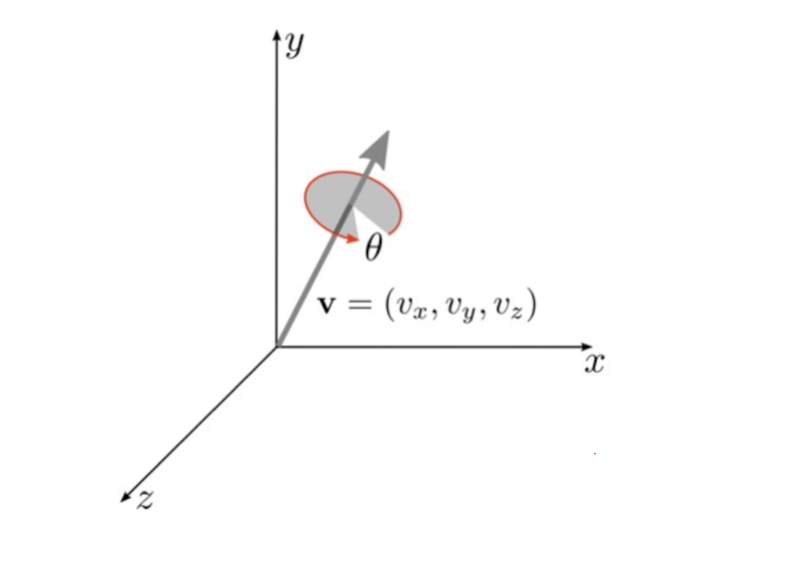
\includegraphics[width=4.16667in,height=\textheight]{images/rotation_abitrary_vector.png}

}

\caption{\label{fig-rot}Rotation around a vector}

\end{figure}

A rotation around \(\vec{r}\) can parameterized with the unit quaternion

\[
  q(\theta, v) = \cos(\frac{\theta}{2}) + i \sin(\frac{\theta}{2}) r_1 +
  j \sin(\frac{\theta}{2}) r_2 + k \sin(\frac{\theta}{2}) r_3 
\]

or componentwise

\[
 q(\theta, v) =  \left(\cos(\frac{\theta}{2}),\; \sin(\frac{\theta}{2})  v_1, \;\sin(\frac{\theta} {2}) v_2, \;\sin(\frac{\theta}{2}) v_3 \right)
\]

The length of \(q\) is
\(||q||=\cos^2(\theta/2) + \sin^2(\theta/2) (v_1^2 + v_2^2 + v_3^2) = \cos^2(\theta/2) + \sin^2(\theta/2) = 1\)

\hypertarget{construction-of-quaternion-from-vector-and-angle}{%
\paragraph{Construction of quaternion from vector and
angle}\label{construction-of-quaternion-from-vector-and-angle}}

Some special quaternions. The yawing can be described by a rotation of
\(\theta\) around the vector \(\vec{r} = (0,0,1)\) and is given by

\[
q_{\text yaw} = (\cos(\frac{\theta}{2}) \theta, 0, 0, \sin(\frac{1}{2} \theta))
\]

The identity be constructed with \(\theta=0\) about any axis
\(q(0) = (\cos(0), v_1 \sin(0), v_2 \sin(0), v_3 \sin(0) = (1,0,0,0)\).

\hypertarget{quaterion-algebra}{%
\subsubsection{Quaterion Algebra}\label{quaterion-algebra}}

\begin{itemize}
\item
  Addition (easy but no geometeric interpretation), just for reference
  \[
  q + p = p + q =  q_w + p_w + (q_1 + p_1) i + (q_2 + p_2) j + (q_3 + p_3) k
  \]
\item
  Multiplication: The multiplication is not commutative \[
  q * p \ne p * q = \tt{Complicated Formula}
  \]
\item
  Conjugate (just i --\textgreater{} -i same for j and k) \[
  q^* = q_w − i q_x − j q_y − k q_z
  \]
\item
  Inverse (in gernal) \[
  q^{-1} = q^*/||q||
  \]
\item
  Inverse (in for rotation quaternions)
\end{itemize}

\[
q^{-1}=q^*
\]

So for unit quaternions, you just have to conjugate to get the inverse.
Luckily, we don't have to remember the formulaes and can use the
onion-package.

\hypertarget{constructing-a-rotation-matrix-from-quaterions-first-solution}{%
\subsubsection{Constructing a rotation matrix from Quaterions (first
solution)}\label{constructing-a-rotation-matrix-from-quaterions-first-solution}}

It's possible to translate the quaternions back to a rotation matrix,
see
\href{https://github.com/oduerr/gesture/blob/main/R/rotation_utils.R}{quat\_to\_mat}.
The code has been taken
\href{https://automaticaddison.com/how-to-convert-a-quaternion-to-a-rotation-matrix/}{from}
We can construct our yaw matrix via

\begin{Shaded}
\begin{Highlighting}[]
\NormalTok{  q01 }\OtherTok{=} \FunctionTok{c}\NormalTok{(}\FunctionTok{cos}\NormalTok{(yaw}\SpecialCharTok{/}\DecValTok{2}\NormalTok{), }\DecValTok{0}\NormalTok{, }\DecValTok{0}\NormalTok{, }\DecValTok{1} \SpecialCharTok{*} \FunctionTok{sin}\NormalTok{(yaw}\SpecialCharTok{/}\DecValTok{2}\NormalTok{))}
  \CommentTok{\#sum(q01\^{}2) \#1}
  \FunctionTok{quat\_to\_mat}\NormalTok{(q01)}
\end{Highlighting}
\end{Shaded}

\begin{verbatim}
          [,1]       [,2] [,3]
[1,] 0.5000000 -0.8660254    0
[2,] 0.8660254  0.5000000    0
[3,] 0.0000000  0.0000000    1
\end{verbatim}

\begin{Shaded}
\begin{Highlighting}[]
  \FunctionTok{Rz}\NormalTok{(yaw)}
\end{Highlighting}
\end{Shaded}

\begin{verbatim}
          [,1]       [,2] [,3]
[1,] 0.5000000 -0.8660254    0
[2,] 0.8660254  0.5000000    0
[3,] 0.0000000  0.0000000    1
\end{verbatim}

\hypertarget{chaining-rotations-with-quaterions-just-multiply-them}{%
\subsubsection{Chaining rotations with quaterions (just multiply
them)}\label{chaining-rotations-with-quaterions-just-multiply-them}}

Now comes properly the most useful thing, that successive rotations can
be done by multiplying the respective quaternions. Let's try this out,
and move the rabit. Note we are still considering body to lab rotations.

Let's multiply several quaternions. We start with \(q_0 = (1,0,0,0)\).

\begin{Shaded}
\begin{Highlighting}[]
\NormalTok{  q0 }\OtherTok{=}\NormalTok{ onion}\SpecialCharTok{::}\FunctionTok{quaternion}\NormalTok{(}\AttributeTok{Re =} \DecValTok{1}\NormalTok{)}
  \FunctionTok{p3d}\NormalTok{(rabbit }\SpecialCharTok{\%*\%} \FunctionTok{quat\_to\_mat}\NormalTok{(q0), }\AttributeTok{h=}\ConstantTok{NULL}\NormalTok{, }\AttributeTok{main =} \StringTok{\textquotesingle{}q0\textquotesingle{}}\NormalTok{)}
\end{Highlighting}
\end{Shaded}

\begin{figure}[H]

{\centering 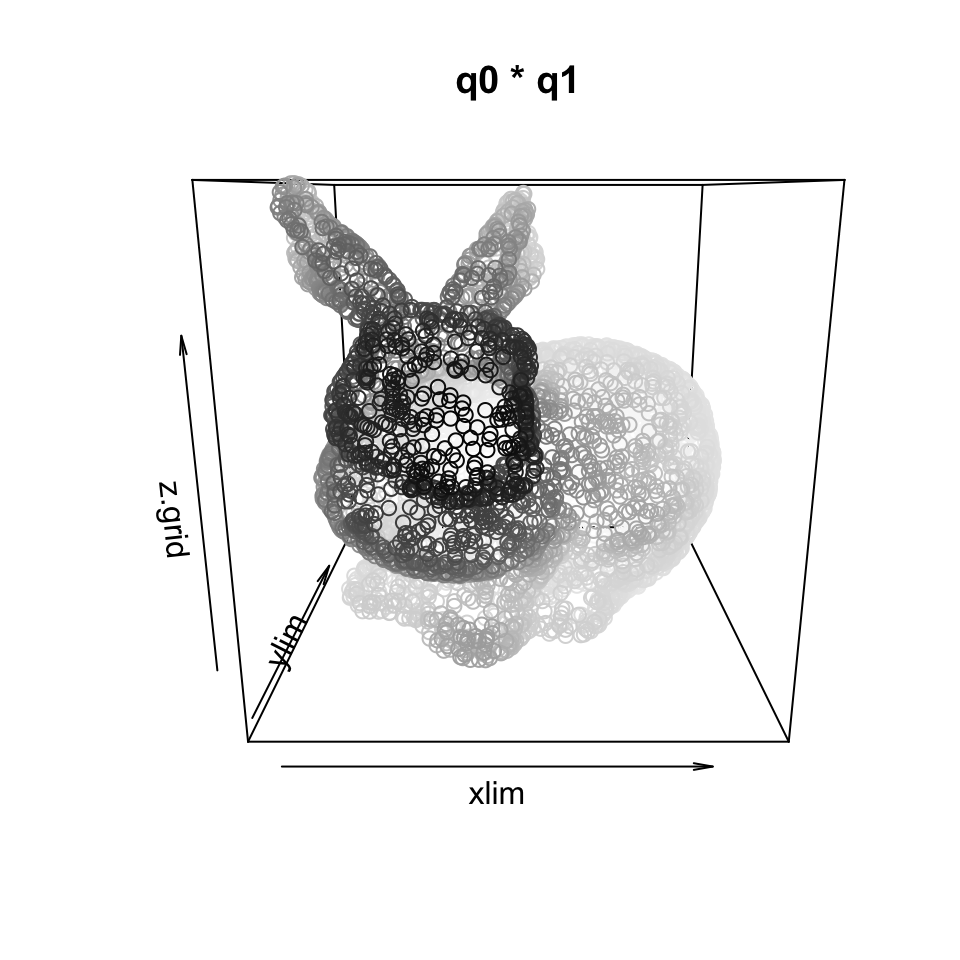
\includegraphics{Note_on_Quaternion_files/figure-pdf/unnamed-chunk-18-1.pdf}

}

\end{figure}

We add a second rotation (a first real) around the z-axis.

\begin{Shaded}
\begin{Highlighting}[]
\NormalTok{  q1 }\OtherTok{=} \FunctionTok{quaternion}\NormalTok{(}\AttributeTok{Re=}\FunctionTok{cos}\NormalTok{(}\SpecialCharTok{{-}}\DecValTok{45}\SpecialCharTok{/}\DecValTok{360} \SpecialCharTok{*}\NormalTok{pi), }\AttributeTok{i =} \DecValTok{0}\NormalTok{, }\AttributeTok{j =} \DecValTok{0}\NormalTok{, }\AttributeTok{k =} \DecValTok{1}\SpecialCharTok{*}\FunctionTok{sin}\NormalTok{(}\SpecialCharTok{{-}}\DecValTok{45}\SpecialCharTok{/}\DecValTok{360} \SpecialCharTok{*}\NormalTok{pi)) }
  \FunctionTok{p3d}\NormalTok{(rabbit }\SpecialCharTok{\%*\%} \FunctionTok{quat\_to\_mat}\NormalTok{(q0 }\SpecialCharTok{*}\NormalTok{ q1), }\AttributeTok{h=}\ConstantTok{NULL}\NormalTok{, }\AttributeTok{main =} \StringTok{\textquotesingle{}q0 * q1\textquotesingle{}}\NormalTok{) }
\end{Highlighting}
\end{Shaded}

\begin{figure}[H]

{\centering 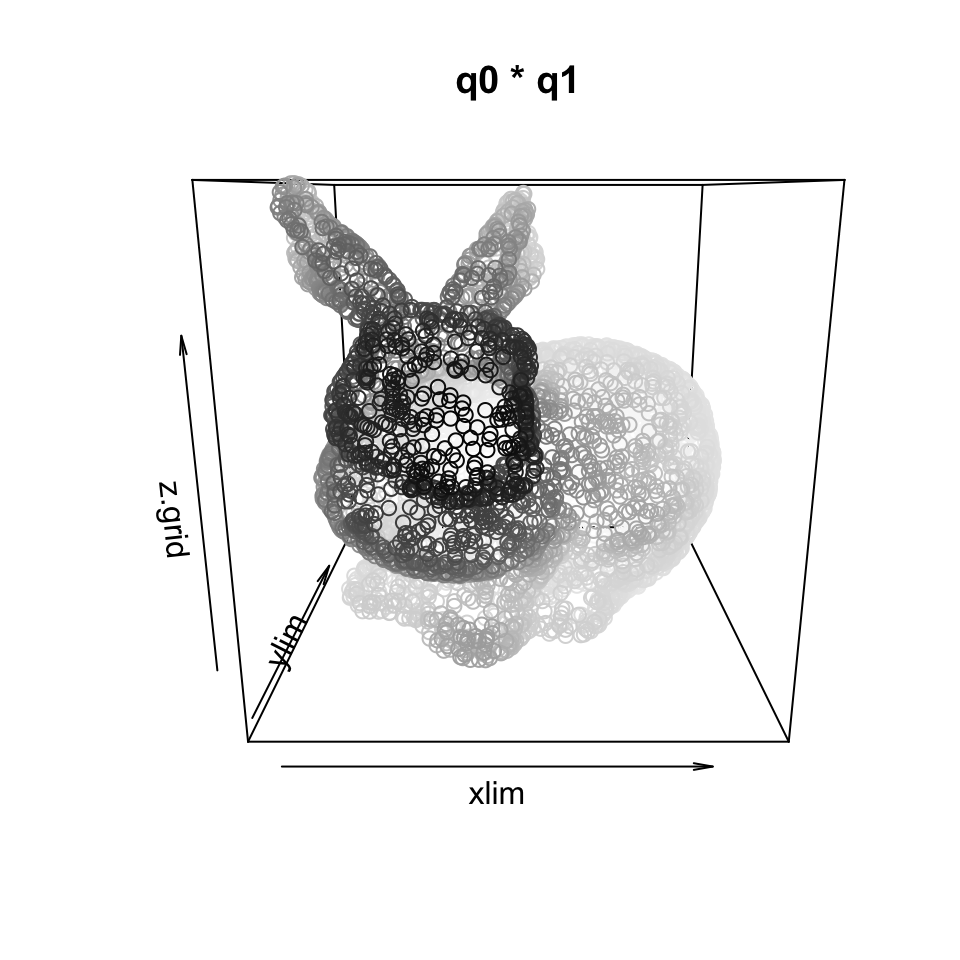
\includegraphics{Note_on_Quaternion_files/figure-pdf/unnamed-chunk-20-1.pdf}

}

\end{figure}

We add a third rotation around the x-axis.

\begin{Shaded}
\begin{Highlighting}[]
\NormalTok{  q2 }\OtherTok{=} \FunctionTok{quaternion}\NormalTok{(}\AttributeTok{Re=}\FunctionTok{cos}\NormalTok{(}\SpecialCharTok{{-}}\DecValTok{45}\SpecialCharTok{/}\DecValTok{360} \SpecialCharTok{*}\NormalTok{pi), }\AttributeTok{i =} \DecValTok{1}\SpecialCharTok{*}\FunctionTok{sin}\NormalTok{(}\SpecialCharTok{{-}}\DecValTok{45}\SpecialCharTok{/}\DecValTok{360} \SpecialCharTok{*}\NormalTok{pi), }\AttributeTok{j =} \DecValTok{0}\NormalTok{, }\AttributeTok{k =} \DecValTok{0}\NormalTok{) }
\NormalTok{  q012 }\OtherTok{=}\NormalTok{ q0 }\SpecialCharTok{*}\NormalTok{ q1 }\SpecialCharTok{*}\NormalTok{ q2 }
  \FunctionTok{p3d}\NormalTok{(rabbit }\SpecialCharTok{\%*\%} \FunctionTok{quat\_to\_mat}\NormalTok{(q012), }\AttributeTok{h=}\ConstantTok{NULL}\NormalTok{, }\AttributeTok{main =} \StringTok{\textquotesingle{}q0 * q1 * q2\textquotesingle{}}\NormalTok{)}
\end{Highlighting}
\end{Shaded}

\begin{figure}[H]

{\centering 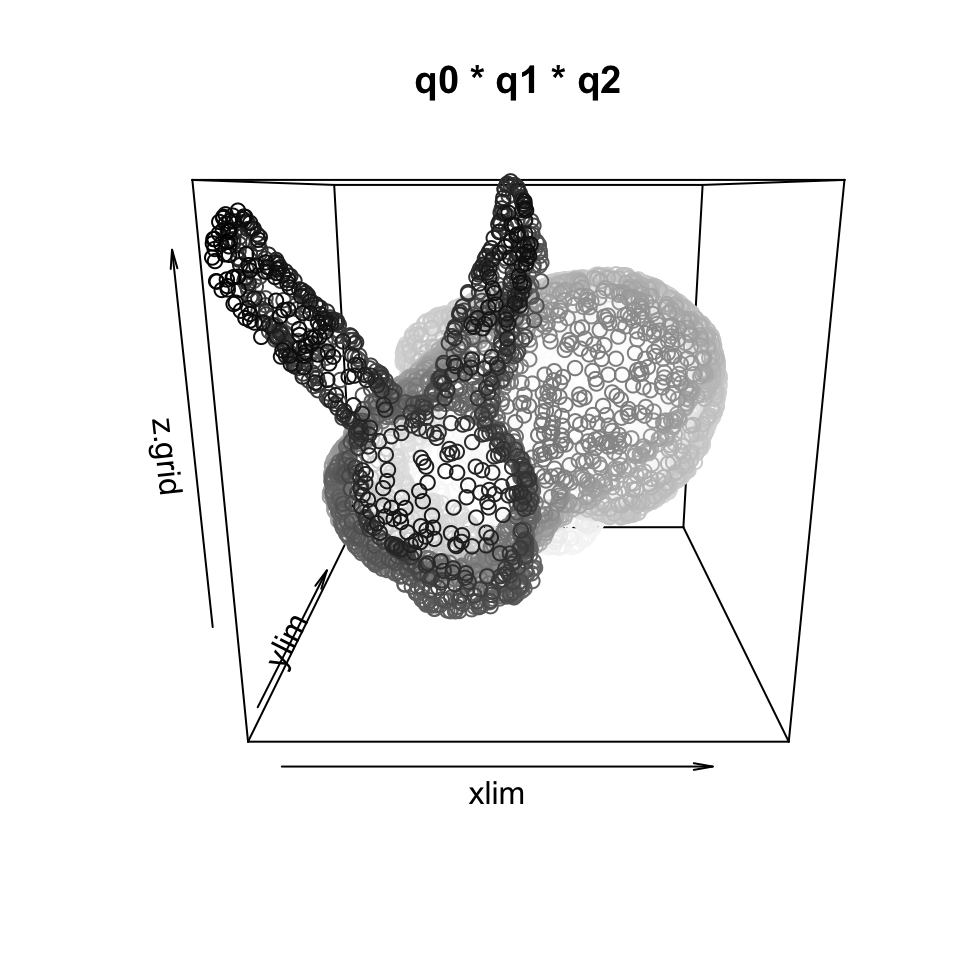
\includegraphics{Note_on_Quaternion_files/figure-pdf/bunny3-1.pdf}

}

\end{figure}

Using the order \(q_0 q_1 q_2\) you transfer the data of the bunny into
the lab frame.

\begin{tcolorbox}[enhanced jigsaw, opacitybacktitle=0.6, rightrule=.15mm, breakable, bottomtitle=1mm, arc=.35mm, colframe=quarto-callout-important-color-frame, coltitle=black, leftrule=.75mm, title=\textcolor{quarto-callout-important-color}{\faExclamation}\hspace{0.5em}{Important}, left=2mm, toptitle=1mm, colbacktitle=quarto-callout-important-color!10!white, titlerule=0mm, colback=white, bottomrule=.15mm, toprule=.15mm, opacityback=0]
Quanternions multiply from left to right
\end{tcolorbox}

\hypertarget{pure-quaternions-real-part-0}{%
\subsubsection{Pure Quaternions (real part =
0)}\label{pure-quaternions-real-part-0}}

We can also use quaterions to transform vectors, without the need to
explicitly construct the rotation matrix as done with the bunny data
above. This is done with so-called \textbf{unit} or \textbf{vector
quaternions}. To obtain a vector quaternions, we set the real part to 0
and use the vector in space as the vector part. That is a vector
\(\vec{v}\) in a certain direction without coding a rotation. From this
vector, we like to know the position to which it gets rotated by
\(R(q) \vec{v}\) the rotation matrix \(R(q)\) corresponding to \(q\). It
can be shown that this is

\[
  (0, R(q) \vec{v}) = q \cdot (0,\vec{v}) \cdot q^{*} 
\]

\begin{Shaded}
\begin{Highlighting}[]
\NormalTok{ q }\OtherTok{=}\NormalTok{ q0 }\SpecialCharTok{*}\NormalTok{ q1 }\SpecialCharTok{*}\NormalTok{ q2 }\CommentTok{\#A unit quaterion defining the direction}
\NormalTok{ vec }\OtherTok{=} \FunctionTok{matrix}\NormalTok{(}\FunctionTok{c}\NormalTok{(}\DecValTok{12}\NormalTok{,}\DecValTok{13}\NormalTok{,}\DecValTok{45}\NormalTok{), }\AttributeTok{ncol=}\DecValTok{1}\NormalTok{) }\CommentTok{\#A vector with which we do the }
 \FunctionTok{quat\_to\_mat}\NormalTok{(q) }\SpecialCharTok{\%*\%}\NormalTok{ vec}
\end{Highlighting}
\end{Shaded}

\begin{verbatim}
         [,1]
[1,] 37.48528
[2,] 20.51472
[3,] 22.62742
\end{verbatim}

\begin{Shaded}
\begin{Highlighting}[]
\NormalTok{ vec\_q }\OtherTok{=} \FunctionTok{quaternion}\NormalTok{(}\AttributeTok{Re =} \DecValTok{0}\NormalTok{, }\AttributeTok{i =}\NormalTok{ vec[}\DecValTok{1}\NormalTok{], }\AttributeTok{j=}\NormalTok{vec[}\DecValTok{2}\NormalTok{], }\AttributeTok{k=}\NormalTok{vec[}\DecValTok{3}\NormalTok{])}
 \CommentTok{\#q\^{}{-}1 is the inverse, which for rotation quaternions is the conjugate }
\NormalTok{ q }\SpecialCharTok{*}\NormalTok{ vec\_q }\SpecialCharTok{*}\NormalTok{ q}\SpecialCharTok{\^{}{-}}\DecValTok{1}
\end{Highlighting}
\end{Shaded}

\begin{verbatim}
              Re
Re -3.552714e-15
i   3.748528e+01
j   2.051472e+01
k   2.262742e+01
\end{verbatim}

TODO build intuition for this expression.

\hypertarget{using-pure-quaterions-to-get-the-rotation-matrix.}{%
\paragraph{Using pure quaterions to get the rotation
matrix.}\label{using-pure-quaterions-to-get-the-rotation-matrix.}}

We can use pure quaterions to get the rotation matrix. To make the
problem harder, we use a more complicated quaternion:

\begin{Shaded}
\begin{Highlighting}[]
\NormalTok{q }\OtherTok{=} \FunctionTok{c}\NormalTok{(}\FloatTok{0.320}\NormalTok{,  }\FloatTok{0.300}\NormalTok{,  }\FloatTok{0.290}\NormalTok{, }\SpecialCharTok{{-}}\FloatTok{0.850}\NormalTok{) }
\NormalTok{q }\OtherTok{=}\NormalTok{ q }\SpecialCharTok{/} \FunctionTok{sqrt}\NormalTok{(}\FunctionTok{sum}\NormalTok{(q}\SpecialCharTok{\^{}}\DecValTok{2}\NormalTok{))}
\NormalTok{q }\OtherTok{=} \FunctionTok{quaternion}\NormalTok{(}\AttributeTok{Re=}\NormalTok{q[}\DecValTok{1}\NormalTok{], }\AttributeTok{i=}\NormalTok{q[}\DecValTok{2}\NormalTok{], }\AttributeTok{j=}\NormalTok{q[}\DecValTok{3}\NormalTok{], }\AttributeTok{k=}\NormalTok{q[}\DecValTok{4}\NormalTok{])}
\FunctionTok{t}\NormalTok{(q}\SpecialCharTok{@}\NormalTok{x)}
\end{Highlighting}
\end{Shaded}

\begin{verbatim}
            Re         i         j          k
[1,] 0.3201601 0.3001501 0.2901451 -0.8504253
\end{verbatim}

We use the fact that the transformation is given by the results of the
unit vectors of the from coordinate system:

\begin{Shaded}
\begin{Highlighting}[]
 \FunctionTok{round}\NormalTok{(}\FunctionTok{quat\_to\_mat}\NormalTok{(q), }\DecValTok{4}\NormalTok{)}
\end{Highlighting}
\end{Shaded}

\begin{verbatim}
        [,1]    [,2]    [,3]
[1,] -0.6148  0.7187 -0.3247
[2,] -0.3704 -0.6266 -0.6857
[3,] -0.6963 -0.3013  0.6515
\end{verbatim}

\begin{Shaded}
\begin{Highlighting}[]
\NormalTok{ e1b }\OtherTok{=}\NormalTok{ q }\SpecialCharTok{*} \FunctionTok{quaternion}\NormalTok{(}\AttributeTok{Re =} \DecValTok{0}\NormalTok{, }\AttributeTok{i =} \DecValTok{1}\NormalTok{) }\SpecialCharTok{*}\NormalTok{ q}\SpecialCharTok{\^{}{-}}\DecValTok{1} 
\NormalTok{ e2b }\OtherTok{=}\NormalTok{ q }\SpecialCharTok{*} \FunctionTok{quaternion}\NormalTok{(}\AttributeTok{Re =} \DecValTok{0}\NormalTok{, }\AttributeTok{j =} \DecValTok{1}\NormalTok{) }\SpecialCharTok{*}\NormalTok{ q}\SpecialCharTok{\^{}{-}}\DecValTok{1} 
\NormalTok{ e3b }\OtherTok{=}\NormalTok{ q }\SpecialCharTok{*} \FunctionTok{quaternion}\NormalTok{(}\AttributeTok{Re =} \DecValTok{0}\NormalTok{, }\AttributeTok{k =} \DecValTok{1}\NormalTok{) }\SpecialCharTok{*}\NormalTok{ q}\SpecialCharTok{\^{}{-}}\DecValTok{1} 
 \FunctionTok{matrix}\NormalTok{(}\FunctionTok{c}\NormalTok{(}
\NormalTok{          e1b}\SpecialCharTok{@}\NormalTok{x[}\DecValTok{2}\SpecialCharTok{:}\DecValTok{4}\NormalTok{],}
\NormalTok{          e2b}\SpecialCharTok{@}\NormalTok{x[}\DecValTok{2}\SpecialCharTok{:}\DecValTok{4}\NormalTok{],}
\NormalTok{          e3b}\SpecialCharTok{@}\NormalTok{x[}\DecValTok{2}\SpecialCharTok{:}\DecValTok{4}\NormalTok{])}
\NormalTok{ ,}\AttributeTok{nrow=}\DecValTok{3}\NormalTok{) }\SpecialCharTok{\%\textgreater{}\%} \FunctionTok{round}\NormalTok{(}\DecValTok{4}\NormalTok{)}
\end{Highlighting}
\end{Shaded}

\begin{verbatim}
        [,1]    [,2]    [,3]
[1,] -0.6148  0.7187 -0.3247
[2,] -0.3704 -0.6266 -0.6857
[3,] -0.6963 -0.3013  0.6515
\end{verbatim}

\hypertarget{todo-flight-coordinates-from-quaterions}{%
\subsubsection{TODO Flight Coordinates from
Quaterions}\label{todo-flight-coordinates-from-quaterions}}

In the definition above has defined as

\[
  R_{\text{Lab} \leftarrow \text{Body}} =  R_{roll} \, R_{pitch}\, R_{yaw} 
\]

\begin{Shaded}
\begin{Highlighting}[]
\NormalTok{  qyaw }\OtherTok{=} \FunctionTok{quaternion}\NormalTok{(}\AttributeTok{Re=}\FunctionTok{cos}\NormalTok{(yaw}\SpecialCharTok{/}\DecValTok{2}\NormalTok{), }\AttributeTok{i=}\DecValTok{0}\NormalTok{,}\AttributeTok{j=}\DecValTok{0}\NormalTok{,}\AttributeTok{k=}\FunctionTok{sin}\NormalTok{(yaw}\SpecialCharTok{/}\DecValTok{2}\NormalTok{))}
\NormalTok{  qpitch }\OtherTok{=} \FunctionTok{quaternion}\NormalTok{(}\AttributeTok{Re=}\FunctionTok{cos}\NormalTok{(pitch}\SpecialCharTok{/}\DecValTok{2}\NormalTok{), }\AttributeTok{i=}\DecValTok{0}\NormalTok{,}\AttributeTok{j=}\FunctionTok{sin}\NormalTok{(pitch}\SpecialCharTok{/}\DecValTok{2}\NormalTok{),}\AttributeTok{k=}\DecValTok{0}\NormalTok{)}
\NormalTok{  qroll }\OtherTok{=} \FunctionTok{quaternion}\NormalTok{(}\AttributeTok{Re=}\FunctionTok{cos}\NormalTok{(roll}\SpecialCharTok{/}\DecValTok{2}\NormalTok{), }\AttributeTok{i=}\FunctionTok{sin}\NormalTok{(roll}\SpecialCharTok{/}\DecValTok{2}\NormalTok{), }\AttributeTok{j=}\DecValTok{0}\NormalTok{,}\AttributeTok{k=}\DecValTok{0}\NormalTok{)}
  \ControlFlowTok{if}\NormalTok{ (}\ConstantTok{FALSE}\NormalTok{) \{ }\CommentTok{\#For debugging}
    \FunctionTok{sum}\NormalTok{(qyaw}\SpecialCharTok{@}\NormalTok{x}\SpecialCharTok{\^{}}\DecValTok{2}\NormalTok{) }\CommentTok{\#1}
    \FunctionTok{sum}\NormalTok{(qpitch}\SpecialCharTok{@}\NormalTok{x}\SpecialCharTok{\^{}}\DecValTok{2}\NormalTok{) }\CommentTok{\#1}
    \FunctionTok{sum}\NormalTok{(qroll}\SpecialCharTok{@}\NormalTok{x}\SpecialCharTok{\^{}}\DecValTok{2}\NormalTok{) }\CommentTok{\#1}
    \CommentTok{\#R = R.roll \%*\% R.pitch \%*\% R.yaw}
    \FunctionTok{sum}\NormalTok{((}\FunctionTok{quat\_to\_mat}\NormalTok{(qyaw) }\SpecialCharTok{{-}}\NormalTok{ R.yaw)}\SpecialCharTok{\^{}}\DecValTok{2}\NormalTok{) }\CommentTok{\#2.46519e{-}32}
    \FunctionTok{sum}\NormalTok{((}\FunctionTok{quat\_to\_mat}\NormalTok{(qpitch) }\SpecialCharTok{{-}}\NormalTok{ R.pitch)}\SpecialCharTok{\^{}}\DecValTok{2}\NormalTok{) }\CommentTok{\#2.46519e{-}32}
    \FunctionTok{sum}\NormalTok{((}\FunctionTok{quat\_to\_mat}\NormalTok{(qroll) }\SpecialCharTok{{-}}\NormalTok{ R.roll)}\SpecialCharTok{\^{}}\DecValTok{2}\NormalTok{) }\CommentTok{\#4.930381e{-}32}
\NormalTok{  \}}
\NormalTok{  qcomb\_body\_to\_lab }\OtherTok{=}\NormalTok{ qyaw }\SpecialCharTok{*}\NormalTok{ qpitch }\SpecialCharTok{*}\NormalTok{ qroll}
\NormalTok{  qcomb\_lab\_to\_body }\OtherTok{=}\NormalTok{ qcomb\_body\_to\_lab}\SpecialCharTok{\^{}{-}}\DecValTok{1}
  \FunctionTok{max}\NormalTok{(}\FunctionTok{abs}\NormalTok{(R }\SpecialCharTok{{-}} \FunctionTok{quat\_to\_mat}\NormalTok{(qcomb\_body\_to\_lab))) }\CommentTok{\#1.4}
\end{Highlighting}
\end{Shaded}

\begin{verbatim}
[1] 1.029303
\end{verbatim}

\begin{Shaded}
\begin{Highlighting}[]
  \FunctionTok{max}\NormalTok{(}\FunctionTok{abs}\NormalTok{(R }\SpecialCharTok{{-}} \FunctionTok{quat\_to\_mat}\NormalTok{(qcomb\_lab\_to\_body))) }\CommentTok{\#0}
\end{Highlighting}
\end{Shaded}

\begin{verbatim}
[1] 1.532089
\end{verbatim}

\begin{Shaded}
\begin{Highlighting}[]
  \CommentTok{\#{-}{-}{-}\textgreater{} Quat\_to\_}
\end{Highlighting}
\end{Shaded}

Testing the package

The following

\begin{Shaded}
\begin{Highlighting}[]
\NormalTok{quart\_to\_ypr }\OtherTok{=} \ControlFlowTok{function}\NormalTok{(q\_body2lab)\{}
\NormalTok{    q }\OtherTok{=}\NormalTok{ q\_body2lab}
\NormalTok{    w }\OtherTok{=}\NormalTok{ q[}\DecValTok{1}\NormalTok{]}
\NormalTok{    x }\OtherTok{=}\NormalTok{ q[}\DecValTok{2}\NormalTok{]}
\NormalTok{    y }\OtherTok{=}\NormalTok{ q[}\DecValTok{3}\NormalTok{]}
\NormalTok{    z }\OtherTok{=}\NormalTok{ q[}\DecValTok{4}\NormalTok{]}
\NormalTok{    roll }\OtherTok{=} \FunctionTok{atan2}\NormalTok{(}\DecValTok{2} \SpecialCharTok{*}\NormalTok{ (w }\SpecialCharTok{*}\NormalTok{ x }\SpecialCharTok{+}\NormalTok{ y }\SpecialCharTok{*}\NormalTok{ z), }\DecValTok{1} \SpecialCharTok{{-}} \DecValTok{2} \SpecialCharTok{*}\NormalTok{ (x }\SpecialCharTok{*}\NormalTok{ x }\SpecialCharTok{+}\NormalTok{ y }\SpecialCharTok{*}\NormalTok{ y))}
\NormalTok{    pitch }\OtherTok{=} \FunctionTok{asin}\NormalTok{(}\DecValTok{2} \SpecialCharTok{*}\NormalTok{ (w }\SpecialCharTok{*}\NormalTok{ y }\SpecialCharTok{{-}}\NormalTok{ x }\SpecialCharTok{*}\NormalTok{ z))}
\NormalTok{    yaw }\OtherTok{=} \FunctionTok{atan2}\NormalTok{(}\DecValTok{2} \SpecialCharTok{*}\NormalTok{ (w }\SpecialCharTok{*}\NormalTok{ z }\SpecialCharTok{+}\NormalTok{ x }\SpecialCharTok{*}\NormalTok{ y), }\DecValTok{1} \SpecialCharTok{{-}} \DecValTok{2} \SpecialCharTok{*}\NormalTok{ (z }\SpecialCharTok{*}\NormalTok{ z }\SpecialCharTok{+}\NormalTok{ y }\SpecialCharTok{*}\NormalTok{ y))}
    \FunctionTok{return}\NormalTok{(}\FunctionTok{c}\NormalTok{(yaw,pitch,roll))}
\NormalTok{\}}
\FunctionTok{quart\_to\_ypr}\NormalTok{(qcomb\_lab\_to\_body}\SpecialCharTok{@}\NormalTok{x) }\CommentTok{\#Wrong }
\end{Highlighting}
\end{Shaded}

\begin{verbatim}
[1] -1.2311588 -0.2663981 -1.0351367
\end{verbatim}

\begin{Shaded}
\begin{Highlighting}[]
\FunctionTok{quart\_to\_ypr}\NormalTok{(qcomb\_body\_to\_lab}\SpecialCharTok{@}\NormalTok{x) }\CommentTok{\#Correct}
\end{Highlighting}
\end{Shaded}

\begin{verbatim}
[1]  1.0471976 -0.8726646  0.6981317
\end{verbatim}

\begin{Shaded}
\begin{Highlighting}[]
\FunctionTok{c}\NormalTok{(yaw, pitch, roll)}
\end{Highlighting}
\end{Shaded}

\begin{verbatim}
[1]  1.0471976 -0.8726646  0.6981317
\end{verbatim}

\begin{Shaded}
\begin{Highlighting}[]
\CommentTok{\#As it is currently implented}
\NormalTok{dmpGetGravity }\OtherTok{=} \ControlFlowTok{function}\NormalTok{(q)\{}
\NormalTok{  qw }\OtherTok{=}\NormalTok{ q[}\DecValTok{1}\NormalTok{]}
\NormalTok{  qx }\OtherTok{=}\NormalTok{ q[}\DecValTok{2}\NormalTok{]}
\NormalTok{  qy }\OtherTok{=}\NormalTok{ q[}\DecValTok{3}\NormalTok{]}
\NormalTok{  qz }\OtherTok{=}\NormalTok{ q[}\DecValTok{4}\NormalTok{]}
\NormalTok{  vx }\OtherTok{=} \DecValTok{2} \SpecialCharTok{*}\NormalTok{ (qx }\SpecialCharTok{*}\NormalTok{ qz }\SpecialCharTok{{-}}\NormalTok{ qw}\SpecialCharTok{*}\NormalTok{qy)}
\NormalTok{  vy }\OtherTok{=} \DecValTok{2} \SpecialCharTok{*}\NormalTok{ (qw }\SpecialCharTok{*}\NormalTok{ qx }\SpecialCharTok{+}\NormalTok{ qy}\SpecialCharTok{*}\NormalTok{qz)}
\NormalTok{  vz }\OtherTok{=}\NormalTok{ qw}\SpecialCharTok{\^{}}\DecValTok{2} \SpecialCharTok{{-}}\NormalTok{ qx}\SpecialCharTok{\^{}}\DecValTok{2} \SpecialCharTok{{-}}\NormalTok{ qy}\SpecialCharTok{\^{}}\DecValTok{2} \SpecialCharTok{+}\NormalTok{ qz}\SpecialCharTok{\^{}}\DecValTok{2}
  \FunctionTok{return}\NormalTok{(}\FunctionTok{c}\NormalTok{(vx,vy,vz))}
\NormalTok{\}}
\NormalTok{dmpGetYawPitchRoll }\OtherTok{=} \ControlFlowTok{function}\NormalTok{(q, gravity)\{}
\NormalTok{  qw }\OtherTok{=}\NormalTok{ q[}\DecValTok{1}\NormalTok{]}
\NormalTok{  qx }\OtherTok{=}\NormalTok{ q[}\DecValTok{2}\NormalTok{]}
\NormalTok{  qy }\OtherTok{=}\NormalTok{ q[}\DecValTok{3}\NormalTok{]}
\NormalTok{  qz }\OtherTok{=}\NormalTok{ q[}\DecValTok{4}\NormalTok{]}
\NormalTok{  yaw }\OtherTok{=} \FunctionTok{atan2}\NormalTok{(}\DecValTok{2}\SpecialCharTok{*}\NormalTok{qx}\SpecialCharTok{*}\NormalTok{qy }\SpecialCharTok{{-}} \DecValTok{2}\SpecialCharTok{*}\NormalTok{qw}\SpecialCharTok{*}\NormalTok{qz, }\DecValTok{2}\SpecialCharTok{*}\NormalTok{qw}\SpecialCharTok{*}\NormalTok{qw}\SpecialCharTok{+}\DecValTok{2}\SpecialCharTok{*}\NormalTok{qx}\SpecialCharTok{*}\NormalTok{qx}\DecValTok{{-}1}\NormalTok{)}
\NormalTok{  pitch }\OtherTok{=} \FunctionTok{atan}\NormalTok{(gravity[}\DecValTok{1}\NormalTok{]}\SpecialCharTok{/}\FunctionTok{sqrt}\NormalTok{(gravity[}\DecValTok{2}\NormalTok{]}\SpecialCharTok{\^{}}\DecValTok{2}\SpecialCharTok{+}\NormalTok{gravity[}\DecValTok{3}\NormalTok{]}\SpecialCharTok{\^{}}\DecValTok{2}\NormalTok{))}
\NormalTok{  roll }\OtherTok{=} \FunctionTok{atan}\NormalTok{(gravity[}\DecValTok{2}\NormalTok{]}\SpecialCharTok{/}\FunctionTok{sqrt}\NormalTok{(gravity[}\DecValTok{1}\NormalTok{]}\SpecialCharTok{\^{}}\DecValTok{2}\SpecialCharTok{+}\NormalTok{gravity[}\DecValTok{3}\NormalTok{]}\SpecialCharTok{\^{}}\DecValTok{2}\NormalTok{))}
  \FunctionTok{return}\NormalTok{(}\FunctionTok{c}\NormalTok{(yaw, pitch, roll))}
\NormalTok{\}}
\NormalTok{g }\OtherTok{=} \FunctionTok{dmpGetGravity}\NormalTok{(qcomb\_body\_to\_lab}\SpecialCharTok{@}\NormalTok{x)}
\FunctionTok{dmpGetYawPitchRoll}\NormalTok{(qcomb\_body\_to\_lab}\SpecialCharTok{@}\NormalTok{x, g)}
\end{Highlighting}
\end{Shaded}

\begin{verbatim}
[1] -1.2311588  0.8726646  0.4259388
\end{verbatim}

\begin{Shaded}
\begin{Highlighting}[]
\NormalTok{g }\OtherTok{=} \FunctionTok{dmpGetGravity}\NormalTok{(qcomb\_lab\_to\_body}\SpecialCharTok{@}\NormalTok{x)}
\FunctionTok{dmpGetYawPitchRoll}\NormalTok{(qcomb\_lab\_to\_body}\SpecialCharTok{@}\NormalTok{x, g)}
\end{Highlighting}
\end{Shaded}

\begin{verbatim}
[1]  1.0471976  0.2663981 -0.9783880
\end{verbatim}

\begin{Shaded}
\begin{Highlighting}[]
\FunctionTok{c}\NormalTok{(yaw, pitch, roll)}
\end{Highlighting}
\end{Shaded}

\begin{verbatim}
[1]  1.0471976 -0.8726646  0.6981317
\end{verbatim}

\hypertarget{rotation-between-two-quaternions.}{%
\subsubsection{Rotation between two
quaternions.}\label{rotation-between-two-quaternions.}}

Consider the two IMUs (like the one on the thumb and the one on the
palm), the orientation of the first (w.r.t. the laboratory system) is
given by \(q_1\) the orientation of the second by \(q_2\). What is the
rotation getting you from hand to palm. The questions is: which rotation
\(q_{12}\) translates between them. So we ask which \(q_12\) fulfills

\[
  q_2 = q_1 \; q_{12} 
\]

Just calculate the inverse of \(q_1\) and you are done

\[
  q_1^{-1} \; q_2 = q_{12}  
\]

\hypertarget{software-package}{%
\subsection{Software package}\label{software-package}}

There are several software packages helping to deal with rotations and
quaterions. Like the onion package in R.

\hypertarget{the-ahrs-python-package}{%
\subsubsection{The AHRS Python Package}\label{the-ahrs-python-package}}

The AHRS package (https://ahrs.readthedocs.io/en/latest/index.html) used
to estimate the rotation of a IMUs (sensors in e.g.~cell phones and
drones), uses quaternion as lot and also provides some basic operations.

\begin{Shaded}
\begin{Highlighting}[]
\ImportTok{from}\NormalTok{ ahrs }\ImportTok{import}\NormalTok{ Quaternion}
\NormalTok{p }\OperatorTok{=}\NormalTok{ Quaternion([}\FloatTok{0.7071}\NormalTok{, }\FloatTok{0.0}\NormalTok{, }\FloatTok{0.7071}\NormalTok{, }\FloatTok{0.0}\NormalTok{])}
\NormalTok{p }
\NormalTok{q }\OperatorTok{=}\NormalTok{ Quaternion([}\DecValTok{0}\NormalTok{, }\FloatTok{0.7071}\NormalTok{, }\FloatTok{0.0}\NormalTok{, }\FloatTok{0.7071}\NormalTok{])}
\NormalTok{p }\OperatorTok{*}\NormalTok{ q }\CommentTok{\#0., 1., 0., 0.}
\NormalTok{q }\OperatorTok{*}\NormalTok{ p }\CommentTok{\#0., 0., 0., 1.}
\NormalTok{q.conj}\CommentTok{\#0., {-}0.70710678, {-}0., {-}0.70710678}
\NormalTok{d }\OperatorTok{=}\NormalTok{ q}\OperatorTok{*}\NormalTok{q.conj }
\NormalTok{d}
\end{Highlighting}
\end{Shaded}

\hypertarget{refs}{}
\begin{CSLReferences}{1}{0}
\leavevmode\vadjust pre{\hypertarget{ref-grossekatthofer2012introduction}{}}%
Großekatthöfer, Karsten, and Zizung Yoon. 2012. {``Introduction into
Quaternions for Spacecraft Attitude Representation.''} \emph{TU Berlin}
16.

\end{CSLReferences}



\end{document}
